\documentclass[twoside]{book}

% Packages required by doxygen
\usepackage{fixltx2e}
\usepackage{calc}
\usepackage{doxygen}
\usepackage[export]{adjustbox} % also loads graphicx
\usepackage{graphicx}
\usepackage[utf8]{inputenc}
\usepackage{makeidx}
\usepackage{multicol}
\usepackage{multirow}
\PassOptionsToPackage{warn}{textcomp}
\usepackage{textcomp}
\usepackage[nointegrals]{wasysym}
\usepackage[table]{xcolor}

% Font selection
\usepackage[T1]{fontenc}
\usepackage[scaled=.90]{helvet}
\usepackage{courier}
\usepackage{amssymb}
\usepackage{sectsty}
\renewcommand{\familydefault}{\sfdefault}
\allsectionsfont{%
  \fontseries{bc}\selectfont%
  \color{darkgray}%
}
\renewcommand{\DoxyLabelFont}{%
  \fontseries{bc}\selectfont%
  \color{darkgray}%
}
\newcommand{\+}{\discretionary{\mbox{\scriptsize$\hookleftarrow$}}{}{}}

% Page & text layout
\usepackage{geometry}
\geometry{%
  a4paper,%
  top=2.5cm,%
  bottom=2.5cm,%
  left=2.5cm,%
  right=2.5cm%
}
\tolerance=750
\hfuzz=15pt
\hbadness=750
\setlength{\emergencystretch}{15pt}
\setlength{\parindent}{0cm}
\setlength{\parskip}{3ex plus 2ex minus 2ex}
\makeatletter
\renewcommand{\paragraph}{%
  \@startsection{paragraph}{4}{0ex}{-1.0ex}{1.0ex}{%
    \normalfont\normalsize\bfseries\SS@parafont%
  }%
}
\renewcommand{\subparagraph}{%
  \@startsection{subparagraph}{5}{0ex}{-1.0ex}{1.0ex}{%
    \normalfont\normalsize\bfseries\SS@subparafont%
  }%
}
\makeatother

% Headers & footers
\usepackage{fancyhdr}
\pagestyle{fancyplain}
\fancyhead[LE]{\fancyplain{}{\bfseries\thepage}}
\fancyhead[CE]{\fancyplain{}{}}
\fancyhead[RE]{\fancyplain{}{\bfseries\leftmark}}
\fancyhead[LO]{\fancyplain{}{\bfseries\rightmark}}
\fancyhead[CO]{\fancyplain{}{}}
\fancyhead[RO]{\fancyplain{}{\bfseries\thepage}}
\fancyfoot[LE]{\fancyplain{}{}}
\fancyfoot[CE]{\fancyplain{}{}}
\fancyfoot[RE]{\fancyplain{}{\bfseries\scriptsize Generated by Doxygen }}
\fancyfoot[LO]{\fancyplain{}{\bfseries\scriptsize Generated by Doxygen }}
\fancyfoot[CO]{\fancyplain{}{}}
\fancyfoot[RO]{\fancyplain{}{}}
\renewcommand{\footrulewidth}{0.4pt}
\renewcommand{\chaptermark}[1]{%
  \markboth{#1}{}%
}
\renewcommand{\sectionmark}[1]{%
  \markright{\thesection\ #1}%
}

% Indices & bibliography
\usepackage{natbib}
\usepackage[titles]{tocloft}
\setcounter{tocdepth}{3}
\setcounter{secnumdepth}{5}
\makeindex

% Hyperlinks (required, but should be loaded last)
\usepackage{ifpdf}
\ifpdf
  \usepackage[pdftex,pagebackref=true]{hyperref}
\else
  \usepackage[ps2pdf,pagebackref=true]{hyperref}
\fi
\hypersetup{%
  colorlinks=true,%
  linkcolor=blue,%
  citecolor=blue,%
  unicode%
}

% Custom commands
\newcommand{\clearemptydoublepage}{%
  \newpage{\pagestyle{empty}\cleardoublepage}%
}

\usepackage{caption}
\captionsetup{labelsep=space,justification=centering,font={bf},singlelinecheck=off,skip=4pt,position=top}

%===== C O N T E N T S =====

\begin{document}

% Titlepage & ToC
\hypersetup{pageanchor=false,
             bookmarksnumbered=true,
             pdfencoding=unicode
            }
\pagenumbering{roman}
\begin{titlepage}
\vspace*{7cm}
\begin{center}%
{\Large My Project }\\
\vspace*{1cm}
{\large Generated by Doxygen 1.8.11}\\
\end{center}
\end{titlepage}
\clearemptydoublepage
\tableofcontents
\clearemptydoublepage
\pagenumbering{arabic}
\hypersetup{pageanchor=true}

%--- Begin generated contents ---
\chapter{Class Index}
\section{Class List}
Here are the classes, structs, unions and interfaces with brief descriptions\+:\begin{DoxyCompactList}
\item\contentsline{section}{\hyperlink{classAirHabitat}{Air\+Habitat} }{\pageref{classAirHabitat}}{}
\item\contentsline{section}{\hyperlink{classAlligator}{Alligator} }{\pageref{classAlligator}}{}
\item\contentsline{section}{\hyperlink{classAnimal}{Animal} }{\pageref{classAnimal}}{}
\item\contentsline{section}{\hyperlink{classAves}{Aves} }{\pageref{classAves}}{}
\item\contentsline{section}{\hyperlink{classCage}{Cage} }{\pageref{classCage}}{}
\item\contentsline{section}{\hyperlink{classCell}{Cell} }{\pageref{classCell}}{}
\item\contentsline{section}{\hyperlink{classCobra}{Cobra} }{\pageref{classCobra}}{}
\item\contentsline{section}{\hyperlink{classCormorant}{Cormorant} }{\pageref{classCormorant}}{}
\item\contentsline{section}{\hyperlink{classDolphin}{Dolphin} }{\pageref{classDolphin}}{}
\item\contentsline{section}{\hyperlink{classDriver}{Driver} }{\pageref{classDriver}}{}
\item\contentsline{section}{\hyperlink{classDuck}{Duck} }{\pageref{classDuck}}{}
\item\contentsline{section}{\hyperlink{classDugong}{Dugong} }{\pageref{classDugong}}{}
\item\contentsline{section}{\hyperlink{classEagle}{Eagle} }{\pageref{classEagle}}{}
\item\contentsline{section}{\hyperlink{classElephant}{Elephant} }{\pageref{classElephant}}{}
\item\contentsline{section}{\hyperlink{classEntrance}{Entrance} }{\pageref{classEntrance}}{}
\item\contentsline{section}{\hyperlink{classExit}{Exit} }{\pageref{classExit}}{}
\item\contentsline{section}{\hyperlink{classFacility}{Facility} }{\pageref{classFacility}}{}
\item\contentsline{section}{\hyperlink{classFlyingAnimal}{Flying\+Animal} }{\pageref{classFlyingAnimal}}{}
\item\contentsline{section}{\hyperlink{classGiraffe}{Giraffe} }{\pageref{classGiraffe}}{}
\item\contentsline{section}{\hyperlink{classGoat}{Goat} }{\pageref{classGoat}}{}
\item\contentsline{section}{\hyperlink{classHabitat}{Habitat} }{\pageref{classHabitat}}{}
\item\contentsline{section}{\hyperlink{classIguana}{Iguana} }{\pageref{classIguana}}{}
\item\contentsline{section}{\hyperlink{classJalak}{Jalak} }{\pageref{classJalak}}{}
\item\contentsline{section}{\hyperlink{classDriver_1_1Kelas}{Driver\+::\+Kelas} }{\pageref{classDriver_1_1Kelas}}{}
\item\contentsline{section}{\hyperlink{classCage_1_1Kelas}{Cage\+::\+Kelas} }{\pageref{classCage_1_1Kelas}}{}
\item\contentsline{section}{\hyperlink{classCell_1_1Kelas}{Cell\+::\+Kelas} }{\pageref{classCell_1_1Kelas}}{}
\item\contentsline{section}{\hyperlink{classKomodo}{Komodo} }{\pageref{classKomodo}}{}
\item\contentsline{section}{\hyperlink{classLandAnimal}{Land\+Animal} }{\pageref{classLandAnimal}}{}
\item\contentsline{section}{\hyperlink{classLandHabitat}{Land\+Habitat} }{\pageref{classLandHabitat}}{}
\item\contentsline{section}{\hyperlink{classLion}{Lion} }{\pageref{classLion}}{}
\item\contentsline{section}{\hyperlink{classMammal}{Mammal} }{\pageref{classMammal}}{}
\item\contentsline{section}{\hyperlink{classOrca}{Orca} }{\pageref{classOrca}}{}
\item\contentsline{section}{\hyperlink{classOwl}{Owl} }{\pageref{classOwl}}{}
\item\contentsline{section}{\hyperlink{classPark}{Park} }{\pageref{classPark}}{}
\item\contentsline{section}{\hyperlink{classParrot}{Parrot} }{\pageref{classParrot}}{}
\item\contentsline{section}{\hyperlink{classPoint}{Point} }{\pageref{classPoint}}{}
\item\contentsline{section}{\hyperlink{classPolarBear}{Polar\+Bear} }{\pageref{classPolarBear}}{}
\item\contentsline{section}{\hyperlink{classRenderable}{Renderable} }{\pageref{classRenderable}}{}
\item\contentsline{section}{\hyperlink{classReptile}{Reptile} }{\pageref{classReptile}}{}
\item\contentsline{section}{\hyperlink{classRestaurant}{Restaurant} }{\pageref{classRestaurant}}{}
\item\contentsline{section}{\hyperlink{classRoad}{Road} }{\pageref{classRoad}}{}
\item\contentsline{section}{\hyperlink{classTiger}{Tiger} }{\pageref{classTiger}}{}
\item\contentsline{section}{\hyperlink{classWalrus}{Walrus} }{\pageref{classWalrus}}{}
\item\contentsline{section}{\hyperlink{classWaterAnimal}{Water\+Animal} }{\pageref{classWaterAnimal}}{}
\item\contentsline{section}{\hyperlink{classWaterHabitat}{Water\+Habitat} }{\pageref{classWaterHabitat}}{}
\item\contentsline{section}{\hyperlink{classZoo}{Zoo} }{\pageref{classZoo}}{}
\end{DoxyCompactList}

\chapter{File Index}
\section{File List}
Here is a list of all files with brief descriptions\+:\begin{DoxyCompactList}
\item\contentsline{section}{animal/\hyperlink{animal_8cpp}{animal.\+cpp} }{\pageref{animal_8cpp}}{}
\item\contentsline{section}{animal/\hyperlink{animal_8h}{animal.\+h} }{\pageref{animal_8h}}{}
\item\contentsline{section}{cage/\hyperlink{cage_8cpp}{cage.\+cpp} }{\pageref{cage_8cpp}}{}
\item\contentsline{section}{cage/\hyperlink{cage_8h}{cage.\+h} }{\pageref{cage_8h}}{}
\item\contentsline{section}{cell/\hyperlink{cell_8cpp}{cell.\+cpp} }{\pageref{cell_8cpp}}{}
\item\contentsline{section}{cell/\hyperlink{cell_8h}{cell.\+h} }{\pageref{cell_8h}}{}
\item\contentsline{section}{driver/\hyperlink{driver_8cpp}{driver.\+cpp} }{\pageref{driver_8cpp}}{}
\item\contentsline{section}{driver/\hyperlink{driver_8h}{driver.\+h} }{\pageref{driver_8h}}{}
\item\contentsline{section}{main/\hyperlink{main_8cpp}{main.\+cpp} }{\pageref{main_8cpp}}{}
\item\contentsline{section}{point/\hyperlink{point_8cpp}{point.\+cpp} }{\pageref{point_8cpp}}{}
\item\contentsline{section}{point/\hyperlink{point_8h}{point.\+h} }{\pageref{point_8h}}{}
\item\contentsline{section}{zoo/\hyperlink{zoo_8cpp}{zoo.\+cpp} }{\pageref{zoo_8cpp}}{}
\item\contentsline{section}{zoo/\hyperlink{zoo_8h}{zoo.\+h} }{\pageref{zoo_8h}}{}
\end{DoxyCompactList}

\chapter{Class Documentation}
\hypertarget{classAnimal}{}\section{Animal Class Reference}
\label{classAnimal}\index{Animal@{Animal}}


{\ttfamily \#include $<$animal.\+h$>$}



Inheritance diagram for Animal\+:
\nopagebreak
\begin{figure}[H]
\begin{center}
\leavevmode
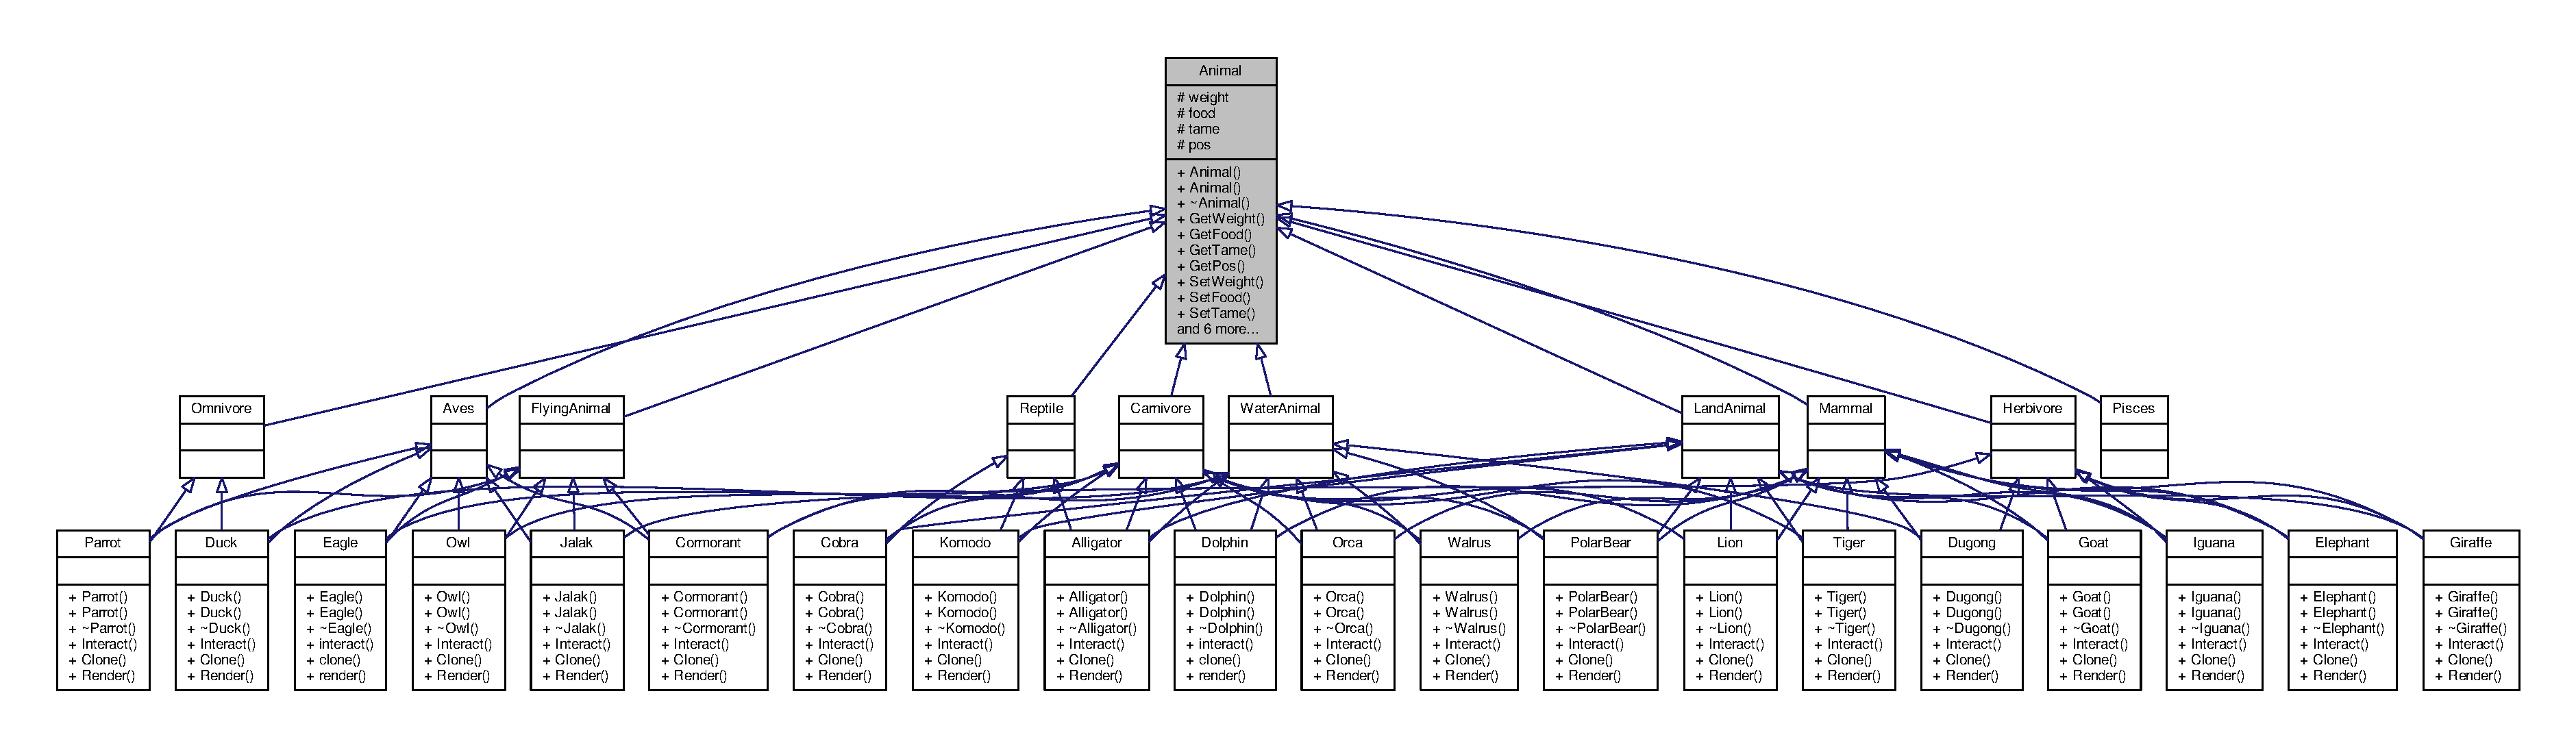
\includegraphics[width=350pt]{classAnimal__inherit__graph}
\end{center}
\end{figure}


Collaboration diagram for Animal\+:
\nopagebreak
\begin{figure}[H]
\begin{center}
\leavevmode
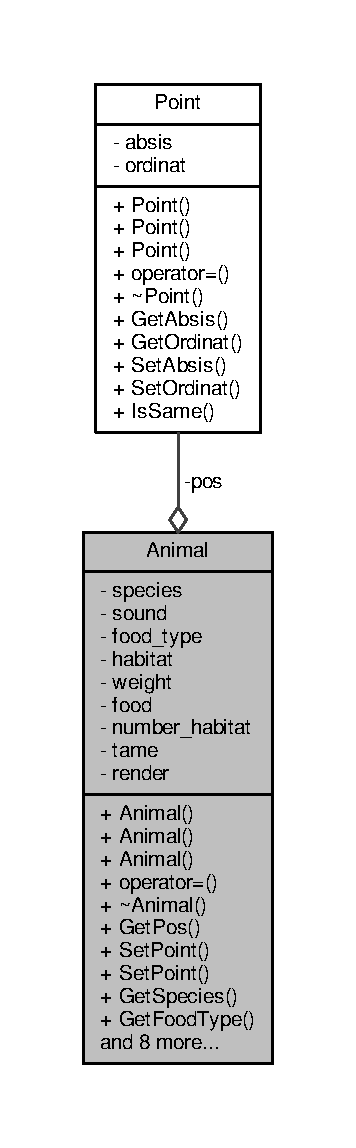
\includegraphics[width=159pt]{classAnimal__coll__graph}
\end{center}
\end{figure}
\subsection*{Public Member Functions}
\begin{DoxyCompactItemize}
\item 
\hyperlink{classAnimal_a1e726a49ec952443190ac62dad22353c}{Animal} ()
\begin{DoxyCompactList}\small\item\em Constructor. Menciptakan \hyperlink{classAnimal}{Animal} kosong. \end{DoxyCompactList}\item 
virtual \hyperlink{classAnimal_a16d8b7f94611cc65f5cdb58cc105527b}{$\sim$\+Animal} ()
\begin{DoxyCompactList}\small\item\em Destructor. \end{DoxyCompactList}\item 
\hyperlink{classPoint}{Point} \hyperlink{classAnimal_a183e4addbbccbe06a77e57bc8893cec1}{Get\+Pos} () const 
\begin{DoxyCompactList}\small\item\em Getter untuk pos. \end{DoxyCompactList}\item 
void \hyperlink{classAnimal_a754c7eb7a8ca6d8bd3e30650546a410d}{Set\+Point} (int abs, int ord)
\begin{DoxyCompactList}\small\item\em Setter point dengan parameter dua buah nilai integer. \end{DoxyCompactList}\item 
void \hyperlink{classAnimal_a02e187a6407bc83c46698544c912be15}{Set\+Point} (const \hyperlink{classPoint}{Point} \&p)
\begin{DoxyCompactList}\small\item\em Setter point dengan parameter sebuah point. \end{DoxyCompactList}\item 
bool \hyperlink{classAnimal_afc66abcbc6efb71c81d5306ea368cffb}{Is\+Same} (const \hyperlink{classAnimal}{Animal} \&a) const 
\begin{DoxyCompactList}\small\item\em Memeriksa kesamaan dua animal. \end{DoxyCompactList}\item 
virtual string \hyperlink{classAnimal_ad5a55fb0355a9425fee6611003d9892c}{Interact} ()=0
\begin{DoxyCompactList}\small\item\em Interaksi yang dilakukan animal. \end{DoxyCompactList}\item 
virtual \hyperlink{classAnimal}{Animal} $\ast$ \hyperlink{classAnimal_a3fc95e2a588b653b9b315e6c7a29c89f}{Clone} () const =0
\begin{DoxyCompactList}\small\item\em Melakukan cloning untuk menciptakan objek \hyperlink{classAnimal}{Animal} baru. \end{DoxyCompactList}\item 
virtual char \hyperlink{classAnimal_a43a47c0f41d211128e04abc6add53def}{Render} ()=0
\begin{DoxyCompactList}\small\item\em Render dari \hyperlink{classAnimal}{Animal}. \end{DoxyCompactList}\end{DoxyCompactItemize}
\subsection*{Protected Attributes}
\begin{DoxyCompactItemize}
\item 
\hyperlink{classPoint}{Point} \hyperlink{classAnimal_ae4e9a6fe53c7ebfbb00536f0e38de5c8}{pos}
\begin{DoxyCompactList}\small\item\em Lokasi binatang. \end{DoxyCompactList}\end{DoxyCompactItemize}


\subsection{Detailed Description}
Kelas abstrak \hyperlink{classAnimal}{Animal} merepresentasikan binatang dalam Virtual \hyperlink{classZoo}{Zoo} 

\subsection{Constructor \& Destructor Documentation}
\index{Animal@{Animal}!Animal@{Animal}}
\index{Animal@{Animal}!Animal@{Animal}}
\subsubsection[{\texorpdfstring{Animal()}{Animal()}}]{\setlength{\rightskip}{0pt plus 5cm}Animal\+::\+Animal (
\begin{DoxyParamCaption}
{}
\end{DoxyParamCaption}
)}\hypertarget{classAnimal_a1e726a49ec952443190ac62dad22353c}{}\label{classAnimal_a1e726a49ec952443190ac62dad22353c}


Constructor. Menciptakan \hyperlink{classAnimal}{Animal} kosong. 

\index{Animal@{Animal}!````~Animal@{$\sim$\+Animal}}
\index{````~Animal@{$\sim$\+Animal}!Animal@{Animal}}
\subsubsection[{\texorpdfstring{$\sim$\+Animal()}{~Animal()}}]{\setlength{\rightskip}{0pt plus 5cm}virtual Animal\+::$\sim$\+Animal (
\begin{DoxyParamCaption}
{}
\end{DoxyParamCaption}
)\hspace{0.3cm}{\ttfamily [inline]}, {\ttfamily [virtual]}}\hypertarget{classAnimal_a16d8b7f94611cc65f5cdb58cc105527b}{}\label{classAnimal_a16d8b7f94611cc65f5cdb58cc105527b}


Destructor. 



\subsection{Member Function Documentation}
\index{Animal@{Animal}!Clone@{Clone}}
\index{Clone@{Clone}!Animal@{Animal}}
\subsubsection[{\texorpdfstring{Clone() const =0}{Clone() const =0}}]{\setlength{\rightskip}{0pt plus 5cm}virtual {\bf Animal}$\ast$ Animal\+::\+Clone (
\begin{DoxyParamCaption}
{}
\end{DoxyParamCaption}
) const\hspace{0.3cm}{\ttfamily [pure virtual]}}\hypertarget{classAnimal_a3fc95e2a588b653b9b315e6c7a29c89f}{}\label{classAnimal_a3fc95e2a588b653b9b315e6c7a29c89f}


Melakukan cloning untuk menciptakan objek \hyperlink{classAnimal}{Animal} baru. 

\begin{DoxyReturn}{Returns}
Mengembalikan pointer to \hyperlink{classAnimal}{Animal} objek tersebut. 
\end{DoxyReturn}


Implemented in \hyperlink{classAlligator_aa317f0d37332919f638128c41cd7b53f}{Alligator}, \hyperlink{classCobra_a1bfd2035a0a700b6362b1853cb12949b}{Cobra}, \hyperlink{classCormorant_a7be371562fab8ab5c2e9e72386ee9aa2}{Cormorant}, \hyperlink{classDolphin_a4be3892432206693d2fae815303e07c4}{Dolphin}, \hyperlink{classDuck_ae3ff98b443c887f37ce63e3ed2e3a690}{Duck}, \hyperlink{classDugong_a8209b4208bd32dfc0fa4e701679306c1}{Dugong}, \hyperlink{classEagle_ace8cb419354688615938d2a53d5c1566}{Eagle}, \hyperlink{classElephant_a723a7c90f44a95d9886163e605aecea7}{Elephant}, \hyperlink{classGiraffe_aa29f8f77477a64fc72f814b7f225c94f}{Giraffe}, \hyperlink{classGoat_a1532200ef20734bb42d0a1306b14d8ad}{Goat}, \hyperlink{classIguana_a40e56fb855d09d2a8788dc73e2fdfc8a}{Iguana}, \hyperlink{classJalak_a85b145221386cdca75274b4438250161}{Jalak}, \hyperlink{classKomodo_aab3bd7ee8235c87e8bbafd8848968be8}{Komodo}, \hyperlink{classLion_ae63405ef106650644a8fcafc7393284e}{Lion}, \hyperlink{classOrca_ac44eb30486ba4051eefa914dc8cd670f}{Orca}, \hyperlink{classOwl_a585e73d53d76b2db489613b7f0b6eecc}{Owl}, \hyperlink{classParrot_aec7fd1385827d67522e1baf3242078b0}{Parrot}, \hyperlink{classPolarBear_aad58cdb9b360996a94f12ade5b6743b7}{Polar\+Bear}, \hyperlink{classTiger_aa376d57a4b2d56edb586f7ba1b170037}{Tiger}, and \hyperlink{classWalrus_a9644eb3d51eb945b716bd37e25c7470e}{Walrus}.

\index{Animal@{Animal}!Get\+Pos@{Get\+Pos}}
\index{Get\+Pos@{Get\+Pos}!Animal@{Animal}}
\subsubsection[{\texorpdfstring{Get\+Pos() const }{GetPos() const }}]{\setlength{\rightskip}{0pt plus 5cm}{\bf Point} Animal\+::\+Get\+Pos (
\begin{DoxyParamCaption}
{}
\end{DoxyParamCaption}
) const}\hypertarget{classAnimal_a183e4addbbccbe06a77e57bc8893cec1}{}\label{classAnimal_a183e4addbbccbe06a77e57bc8893cec1}


Getter untuk pos. 

\begin{DoxyReturn}{Returns}
Mengembalikan nilai lokasi binatang. 
\end{DoxyReturn}
\index{Animal@{Animal}!Interact@{Interact}}
\index{Interact@{Interact}!Animal@{Animal}}
\subsubsection[{\texorpdfstring{Interact()=0}{Interact()=0}}]{\setlength{\rightskip}{0pt plus 5cm}virtual string Animal\+::\+Interact (
\begin{DoxyParamCaption}
{}
\end{DoxyParamCaption}
)\hspace{0.3cm}{\ttfamily [pure virtual]}}\hypertarget{classAnimal_ad5a55fb0355a9425fee6611003d9892c}{}\label{classAnimal_ad5a55fb0355a9425fee6611003d9892c}


Interaksi yang dilakukan animal. 

\begin{DoxyReturn}{Returns}
Mengembalikan string yang merepresentasikan suara \hyperlink{classAnimal}{Animal}. 
\end{DoxyReturn}


Implemented in \hyperlink{classAlligator_a8f6141caa973d33f2066c3561cd817b3}{Alligator}, \hyperlink{classCobra_aa8dd0878e3d654e51bec9592c88bcab5}{Cobra}, \hyperlink{classCormorant_af28984652ae999452d20aed885f0185a}{Cormorant}, \hyperlink{classDolphin_a592506c38c185d7d383ae755deb9bd72}{Dolphin}, \hyperlink{classDuck_a9355aa821755703c02ac96e49692eaea}{Duck}, \hyperlink{classDugong_a861c589c05a791faf03297eb6e718d9e}{Dugong}, \hyperlink{classEagle_a64abae4f80bcdcba7dac9f03126f42aa}{Eagle}, \hyperlink{classElephant_a4f2c4bef5ec886019ee88ad575f94fa7}{Elephant}, \hyperlink{classGiraffe_ad73e5ee5fc62f709c52a1cab68f2a1f3}{Giraffe}, \hyperlink{classGoat_a5f480d88c50724cee8c7a9d18f486144}{Goat}, \hyperlink{classIguana_a271ef320fd3d4973e50e89aa30cffe3e}{Iguana}, \hyperlink{classJalak_a864b931f04f1580759c4a108e1734bb8}{Jalak}, \hyperlink{classKomodo_a250e6b06c369a94faaa551751cd09196}{Komodo}, \hyperlink{classLion_a4c090a9b5f42b92c30d223b40435e167}{Lion}, \hyperlink{classOrca_adf95ca04578ac04aaa717ef2dd11bf4c}{Orca}, \hyperlink{classOwl_ac3c735f8a34b46780a0efd052319e7f3}{Owl}, \hyperlink{classParrot_a3fdf1aa0851d53d31b5d225d755e4995}{Parrot}, \hyperlink{classPolarBear_a2c266e69dd929ac3b10fe7484a77a5a4}{Polar\+Bear}, \hyperlink{classTiger_ae318cc373300a52e13598f42368a2c70}{Tiger}, and \hyperlink{classWalrus_aa21a90ecf8aff97c4cf90a59449ce02c}{Walrus}.

\index{Animal@{Animal}!Is\+Same@{Is\+Same}}
\index{Is\+Same@{Is\+Same}!Animal@{Animal}}
\subsubsection[{\texorpdfstring{Is\+Same(const Animal \&a) const }{IsSame(const Animal &a) const }}]{\setlength{\rightskip}{0pt plus 5cm}bool Animal\+::\+Is\+Same (
\begin{DoxyParamCaption}
\item[{const {\bf Animal} \&}]{a}
\end{DoxyParamCaption}
) const}\hypertarget{classAnimal_afc66abcbc6efb71c81d5306ea368cffb}{}\label{classAnimal_afc66abcbc6efb71c81d5306ea368cffb}


Memeriksa kesamaan dua animal. 


\begin{DoxyParams}{Parameters}
{\em a} & Objek animal yang akan dibandingkan. \\
\hline
\end{DoxyParams}
\begin{DoxyReturn}{Returns}
Mengeluarkan true jika current object sama dengan animal a. 
\end{DoxyReturn}
\index{Animal@{Animal}!Render@{Render}}
\index{Render@{Render}!Animal@{Animal}}
\subsubsection[{\texorpdfstring{Render()=0}{Render()=0}}]{\setlength{\rightskip}{0pt plus 5cm}virtual char Animal\+::\+Render (
\begin{DoxyParamCaption}
{}
\end{DoxyParamCaption}
)\hspace{0.3cm}{\ttfamily [pure virtual]}}\hypertarget{classAnimal_a43a47c0f41d211128e04abc6add53def}{}\label{classAnimal_a43a47c0f41d211128e04abc6add53def}


Render dari \hyperlink{classAnimal}{Animal}. 

\begin{DoxyReturn}{Returns}
Mengembalikan char yang merupakan representasi kode \hyperlink{classAnimal}{Animal}. 
\end{DoxyReturn}


Implemented in \hyperlink{classAlligator_aa8f0a207888bf7f682ebc6b57270dd33}{Alligator}, \hyperlink{classCobra_abca7da2ee55ce825dc49f4f9a3e87208}{Cobra}, \hyperlink{classCormorant_a6d388885acfc98de6020a01b90259dac}{Cormorant}, \hyperlink{classDolphin_aa051d8ebe93c1c11b503ae76d07cd178}{Dolphin}, \hyperlink{classDuck_a8453f95adcf2e7ff1b35a1a9d9948510}{Duck}, \hyperlink{classDugong_af82a8983c960604aa27dabe7fec53362}{Dugong}, \hyperlink{classEagle_a34e512cb19b5ba1f8a7bce937c57f33f}{Eagle}, \hyperlink{classElephant_a7e412f36e1f88cd278dea76d4f383e95}{Elephant}, \hyperlink{classGiraffe_a64dccf030fdb54de9fd37f8381c64271}{Giraffe}, \hyperlink{classGoat_aedea4680fe17571c2f51d35b90397f6e}{Goat}, \hyperlink{classIguana_a18bbb71a80e6b2a9855623b1c7f108b9}{Iguana}, \hyperlink{classJalak_af500189104401b66d6ab4e3b1106ce74}{Jalak}, \hyperlink{classKomodo_a06ce8ed3d58a33968ecf4a12a3ebbd4d}{Komodo}, \hyperlink{classLion_ad782de7c88e4a7aad01287a2ed64827c}{Lion}, \hyperlink{classOrca_a0673bfc8e70af67b463a4fcae224d9d5}{Orca}, \hyperlink{classOwl_ab4ecc1fc8da822f97299709508f7806d}{Owl}, \hyperlink{classParrot_a27c491ab4ae56491fbe8d74e494bc46d}{Parrot}, \hyperlink{classPolarBear_a7feccf8999fb0ab000c052583ad0217a}{Polar\+Bear}, \hyperlink{classTiger_a42b09a0bfc8c115e7383e926513fb371}{Tiger}, and \hyperlink{classWalrus_a143f948e4c45e13a67f893caa435475d}{Walrus}.

\index{Animal@{Animal}!Set\+Point@{Set\+Point}}
\index{Set\+Point@{Set\+Point}!Animal@{Animal}}
\subsubsection[{\texorpdfstring{Set\+Point(int abs, int ord)}{SetPoint(int abs, int ord)}}]{\setlength{\rightskip}{0pt plus 5cm}void Animal\+::\+Set\+Point (
\begin{DoxyParamCaption}
\item[{int}]{abs, }
\item[{int}]{ord}
\end{DoxyParamCaption}
)}\hypertarget{classAnimal_a754c7eb7a8ca6d8bd3e30650546a410d}{}\label{classAnimal_a754c7eb7a8ca6d8bd3e30650546a410d}


Setter point dengan parameter dua buah nilai integer. 


\begin{DoxyParams}{Parameters}
{\em abs} & Nilai absis yang akan di-\/set pada lokasi animal. \\
\hline
{\em ord} & Nilai ordinat yang akan di-\/set pada lokasi animal. \\
\hline
\end{DoxyParams}
\index{Animal@{Animal}!Set\+Point@{Set\+Point}}
\index{Set\+Point@{Set\+Point}!Animal@{Animal}}
\subsubsection[{\texorpdfstring{Set\+Point(const Point \&p)}{SetPoint(const Point &p)}}]{\setlength{\rightskip}{0pt plus 5cm}void Animal\+::\+Set\+Point (
\begin{DoxyParamCaption}
\item[{const {\bf Point} \&}]{p}
\end{DoxyParamCaption}
)}\hypertarget{classAnimal_a02e187a6407bc83c46698544c912be15}{}\label{classAnimal_a02e187a6407bc83c46698544c912be15}


Setter point dengan parameter sebuah point. 


\begin{DoxyParams}{Parameters}
{\em p} & Objek point yang akan di-\/set pada lokasi animal. \\
\hline
\end{DoxyParams}


\subsection{Member Data Documentation}
\index{Animal@{Animal}!pos@{pos}}
\index{pos@{pos}!Animal@{Animal}}
\subsubsection[{\texorpdfstring{pos}{pos}}]{\setlength{\rightskip}{0pt plus 5cm}{\bf Point} Animal\+::pos\hspace{0.3cm}{\ttfamily [protected]}}\hypertarget{classAnimal_ae4e9a6fe53c7ebfbb00536f0e38de5c8}{}\label{classAnimal_ae4e9a6fe53c7ebfbb00536f0e38de5c8}


Lokasi binatang. 



The documentation for this class was generated from the following files\+:\begin{DoxyCompactItemize}
\item 
animal/\hyperlink{animal_8h}{animal.\+h}\item 
animal/\hyperlink{animal_8cpp}{animal.\+cpp}\end{DoxyCompactItemize}

\hypertarget{classCage}{}\section{Cage Class Reference}
\label{classCage}\index{Cage@{Cage}}


{\ttfamily \#include $<$cage.\+h$>$}



Collaboration diagram for Cage\+:
% FIG 0
\subsection*{Classes}
\begin{DoxyCompactItemize}
\item 
class \hyperlink{classCage_1_1Kelas}{Kelas}
\end{DoxyCompactItemize}
\subsection*{Public Member Functions}
\begin{DoxyCompactItemize}
\item 
\hyperlink{classCage_ac03246dd263ee9fe6f37336317e62b69}{Cage} ()
\begin{DoxyCompactList}\small\item\em Constructor. Menciptakan \hyperlink{classCage}{Cage} kosong tanpa animal. \end{DoxyCompactList}\item 
\hyperlink{classCage_a8cd728b1eb23303888a153230f96490e}{Cage} (int s)
\begin{DoxyCompactList}\small\item\em Constructor dengan parameter. Menciptakan \hyperlink{classCage}{Cage} dengan size s tanpa animal. \end{DoxyCompactList}\item 
\hyperlink{classCage_a105ec044af346561cc7165f69da8cf08}{Cage} (int i, int j)
\begin{DoxyCompactList}\small\item\em Constructor. Menciptakan \hyperlink{classCage}{Cage} dengan size 1 dan loc i,j. \end{DoxyCompactList}\item 
\hyperlink{classCage_ae85bb53517616422bf7f36282de01519}{Cage} (const \hyperlink{classCage}{Cage} \&c)
\begin{DoxyCompactList}\small\item\em Copy Constructor. \end{DoxyCompactList}\item 
\hyperlink{classCage}{Cage} \& \hyperlink{classCage_a020eefd2b5d15915cf65693413be64db}{operator=} (const \hyperlink{classCage}{Cage} \&c)
\begin{DoxyCompactList}\small\item\em Operator =. \end{DoxyCompactList}\item 
\hyperlink{classCage_a657259499dfc23c63fc65aeaf8abbb17}{$\sim$\+Cage} ()
\begin{DoxyCompactList}\small\item\em Destructor. \end{DoxyCompactList}\item 
bool \hyperlink{classCage_af244dea5f1b3645d3f216a16f353ddc7}{Is\+Full} () const 
\begin{DoxyCompactList}\small\item\em Is\+Full. Menentukan apakah cage penuh. \end{DoxyCompactList}\item 
int \hyperlink{classCage_abf801136c687ea862b64d0c36a2ce5cd}{Get\+Size} () const 
\begin{DoxyCompactList}\small\item\em Get\+Size. \end{DoxyCompactList}\item 
\hyperlink{classAnimal}{Animal} \hyperlink{classCage_a298833379b741edbdaf5115e4993db1e}{Get\+Animal} (int i) const 
\begin{DoxyCompactList}\small\item\em Get\+Animal. \end{DoxyCompactList}\item 
int \hyperlink{classCage_a49312121ccca0c0b731f3fe1256a28a2}{Get\+Total\+Animal} () const 
\begin{DoxyCompactList}\small\item\em Get\+Total\+Animal. \end{DoxyCompactList}\item 
\hyperlink{classPoint}{Point} \hyperlink{classCage_ae01123979c931296ca477d9d15d9efba}{Get\+Point} (int i) const 
\begin{DoxyCompactList}\small\item\em Get\+Point. \end{DoxyCompactList}\item 
void \hyperlink{classCage_a928e4a1686c1c9ca4f7e703d107de415}{Adopt\+Animal} (\hyperlink{classAnimal}{Animal} A)
\begin{DoxyCompactList}\small\item\em Adopt\+Animal. \end{DoxyCompactList}\item 
void \hyperlink{classCage_a84c0aac0bfd315ef7e5d0595dea5be5a}{Release\+Animal} (int i)
\begin{DoxyCompactList}\small\item\em Release\+Animal. Melepas suatu binatang yang terdapat pada cage. \end{DoxyCompactList}\item 
bool \hyperlink{classCage_a8f2321f5ca7e5fed271350ea1800e10b}{Is\+Empty} () const 
\begin{DoxyCompactList}\small\item\em Is\+Empty. \end{DoxyCompactList}\item 
bool \hyperlink{classCage_aafb5de9009a7ef80fc039f27793c8df6}{Is\+Occupied} (int i) const 
\begin{DoxyCompactList}\small\item\em Is\+Occupied. Menentukan apakah \hyperlink{classCage}{Cage} sudah terisi. \end{DoxyCompactList}\item 
bool \hyperlink{classCage_a176fc9feeb9855881e85c5d8551a6443}{Is\+Occupied} (const \hyperlink{classPoint}{Point} \&p) const 
\begin{DoxyCompactList}\small\item\em Is\+Occupied. Menentukan apakah \hyperlink{classCage}{Cage} sudah terisi. \end{DoxyCompactList}\item 
int \hyperlink{classCage_aaf098729df55f3cf45068d32fe6d5c4b}{Is\+In\+Cage} (const \hyperlink{classAnimal}{Animal} \&A) const 
\begin{DoxyCompactList}\small\item\em Is\+In\+Cage. Menentukan apakah suatu binatang terdapat pada cage. \end{DoxyCompactList}\item 
bool \hyperlink{classCage_a2ac9ea442655213ae3d52a6a7dc30fcf}{Is\+In\+Cage} (const \hyperlink{classPoint}{Point} \&P) const 
\begin{DoxyCompactList}\small\item\em Is\+In\+Cage. Menentukan apakah P terdapat dalam cage. \end{DoxyCompactList}\item 
void \hyperlink{classCage_a78f919dc2b8a3e89a7375c97643a2633}{Interact} () const 
\begin{DoxyCompactList}\small\item\em Interact. Mencetak interaksi animal cage ke layar. \end{DoxyCompactList}\item 
void \hyperlink{classCage_aed8ca487fb22db2ca755bc9d784342fc}{Add\+Point} (\hyperlink{classPoint}{Point} P)
\begin{DoxyCompactList}\small\item\em Add\+Point. Menambahkan Loc baru di dalam \hyperlink{classCage}{Cage}. \end{DoxyCompactList}\item 
bool \hyperlink{classCage_aece0c17d0299b55c596eb68175df71a8}{Can\+Put} (const \hyperlink{classAnimal}{Animal} \&A) const 
\begin{DoxyCompactList}\small\item\em Can\+Put. Menentukan apakah A dapat dimasukkan ke cage. \end{DoxyCompactList}\item 
bool \hyperlink{classCage_a973611397e576888027012237486cd25}{Move} ()
\begin{DoxyCompactList}\small\item\em Move. Menggerakkan semua binatang yang terdapat pada cage. \end{DoxyCompactList}\end{DoxyCompactItemize}


\subsection{Constructor \& Destructor Documentation}
\index{Cage@{Cage}!Cage@{Cage}}
\index{Cage@{Cage}!Cage@{Cage}}
\subsubsection[{\texorpdfstring{Cage()}{Cage()}}]{\setlength{\rightskip}{0pt plus 5cm}Cage\+::\+Cage (
\begin{DoxyParamCaption}
{}
\end{DoxyParamCaption}
)}\hypertarget{classCage_ac03246dd263ee9fe6f37336317e62b69}{}\label{classCage_ac03246dd263ee9fe6f37336317e62b69}


Constructor. Menciptakan \hyperlink{classCage}{Cage} kosong tanpa animal. 

\index{Cage@{Cage}!Cage@{Cage}}
\index{Cage@{Cage}!Cage@{Cage}}
\subsubsection[{\texorpdfstring{Cage(int s)}{Cage(int s)}}]{\setlength{\rightskip}{0pt plus 5cm}Cage\+::\+Cage (
\begin{DoxyParamCaption}
\item[{int}]{s}
\end{DoxyParamCaption}
)}\hypertarget{classCage_a8cd728b1eb23303888a153230f96490e}{}\label{classCage_a8cd728b1eb23303888a153230f96490e}


Constructor dengan parameter. Menciptakan \hyperlink{classCage}{Cage} dengan size s tanpa animal. 


\begin{DoxyParams}{Parameters}
{\em s} & Nilai ukuran \hyperlink{classCage}{Cage}. \\
\hline
\end{DoxyParams}
\index{Cage@{Cage}!Cage@{Cage}}
\index{Cage@{Cage}!Cage@{Cage}}
\subsubsection[{\texorpdfstring{Cage(int i, int j)}{Cage(int i, int j)}}]{\setlength{\rightskip}{0pt plus 5cm}Cage\+::\+Cage (
\begin{DoxyParamCaption}
\item[{int}]{i, }
\item[{int}]{j}
\end{DoxyParamCaption}
)}\hypertarget{classCage_a105ec044af346561cc7165f69da8cf08}{}\label{classCage_a105ec044af346561cc7165f69da8cf08}


Constructor. Menciptakan \hyperlink{classCage}{Cage} dengan size 1 dan loc i,j. 


\begin{DoxyParams}{Parameters}
{\em i} & absis \hyperlink{classPoint}{Point} pada \hyperlink{classCage}{Cage}. \\
\hline
{\em j} & ordinat \hyperlink{classPoint}{Point} pada \hyperlink{classCage}{Cage}. \\
\hline
\end{DoxyParams}
\index{Cage@{Cage}!Cage@{Cage}}
\index{Cage@{Cage}!Cage@{Cage}}
\subsubsection[{\texorpdfstring{Cage(const Cage \&c)}{Cage(const Cage &c)}}]{\setlength{\rightskip}{0pt plus 5cm}Cage\+::\+Cage (
\begin{DoxyParamCaption}
\item[{const {\bf Cage} \&}]{c}
\end{DoxyParamCaption}
)}\hypertarget{classCage_ae85bb53517616422bf7f36282de01519}{}\label{classCage_ae85bb53517616422bf7f36282de01519}


Copy Constructor. 


\begin{DoxyParams}{Parameters}
{\em c} & Objek yang akan di-\/copy. \\
\hline
\end{DoxyParams}
\index{Cage@{Cage}!````~Cage@{$\sim$\+Cage}}
\index{````~Cage@{$\sim$\+Cage}!Cage@{Cage}}
\subsubsection[{\texorpdfstring{$\sim$\+Cage()}{~Cage()}}]{\setlength{\rightskip}{0pt plus 5cm}Cage\+::$\sim$\+Cage (
\begin{DoxyParamCaption}
{}
\end{DoxyParamCaption}
)}\hypertarget{classCage_a657259499dfc23c63fc65aeaf8abbb17}{}\label{classCage_a657259499dfc23c63fc65aeaf8abbb17}


Destructor. 



\subsection{Member Function Documentation}
\index{Cage@{Cage}!Add\+Point@{Add\+Point}}
\index{Add\+Point@{Add\+Point}!Cage@{Cage}}
\subsubsection[{\texorpdfstring{Add\+Point(\+Point P)}{AddPoint(Point P)}}]{\setlength{\rightskip}{0pt plus 5cm}void Cage\+::\+Add\+Point (
\begin{DoxyParamCaption}
\item[{{\bf Point}}]{P}
\end{DoxyParamCaption}
)}\hypertarget{classCage_aed8ca487fb22db2ca755bc9d784342fc}{}\label{classCage_aed8ca487fb22db2ca755bc9d784342fc}


Add\+Point. Menambahkan Loc baru di dalam \hyperlink{classCage}{Cage}. 

\index{Cage@{Cage}!Adopt\+Animal@{Adopt\+Animal}}
\index{Adopt\+Animal@{Adopt\+Animal}!Cage@{Cage}}
\subsubsection[{\texorpdfstring{Adopt\+Animal(\+Animal A)}{AdoptAnimal(Animal A)}}]{\setlength{\rightskip}{0pt plus 5cm}void Cage\+::\+Adopt\+Animal (
\begin{DoxyParamCaption}
\item[{{\bf Animal}}]{A}
\end{DoxyParamCaption}
)}\hypertarget{classCage_a928e4a1686c1c9ca4f7e703d107de415}{}\label{classCage_a928e4a1686c1c9ca4f7e703d107de415}


Adopt\+Animal. 


\begin{DoxyParams}{Parameters}
{\em A} & Objek binatang yang akan dimasukkan. \\
\hline
\end{DoxyParams}
\index{Cage@{Cage}!Can\+Put@{Can\+Put}}
\index{Can\+Put@{Can\+Put}!Cage@{Cage}}
\subsubsection[{\texorpdfstring{Can\+Put(const Animal \&\+A) const }{CanPut(const Animal &A) const }}]{\setlength{\rightskip}{0pt plus 5cm}bool Cage\+::\+Can\+Put (
\begin{DoxyParamCaption}
\item[{const {\bf Animal} \&}]{A}
\end{DoxyParamCaption}
) const}\hypertarget{classCage_aece0c17d0299b55c596eb68175df71a8}{}\label{classCage_aece0c17d0299b55c596eb68175df71a8}


Can\+Put. Menentukan apakah A dapat dimasukkan ke cage. 


\begin{DoxyParams}{Parameters}
{\em A} & \hyperlink{classAnimal}{Animal} yang akan dimasukkan. \\
\hline
\end{DoxyParams}
\begin{DoxyReturn}{Returns}
Mengeluarkan true jika A dapat dimasukkan ke cage. 
\end{DoxyReturn}
\index{Cage@{Cage}!Get\+Animal@{Get\+Animal}}
\index{Get\+Animal@{Get\+Animal}!Cage@{Cage}}
\subsubsection[{\texorpdfstring{Get\+Animal(int i) const }{GetAnimal(int i) const }}]{\setlength{\rightskip}{0pt plus 5cm}{\bf Animal} Cage\+::\+Get\+Animal (
\begin{DoxyParamCaption}
\item[{int}]{i}
\end{DoxyParamCaption}
) const\hspace{0.3cm}{\ttfamily [inline]}}\hypertarget{classCage_a298833379b741edbdaf5115e4993db1e}{}\label{classCage_a298833379b741edbdaf5115e4993db1e}


Get\+Animal. 

\begin{DoxyReturn}{Returns}
Mengembalikan array animal pada \hyperlink{classCage}{Cage}. 
\end{DoxyReturn}
\index{Cage@{Cage}!Get\+Point@{Get\+Point}}
\index{Get\+Point@{Get\+Point}!Cage@{Cage}}
\subsubsection[{\texorpdfstring{Get\+Point(int i) const }{GetPoint(int i) const }}]{\setlength{\rightskip}{0pt plus 5cm}{\bf Point} Cage\+::\+Get\+Point (
\begin{DoxyParamCaption}
\item[{int}]{i}
\end{DoxyParamCaption}
) const\hspace{0.3cm}{\ttfamily [inline]}}\hypertarget{classCage_ae01123979c931296ca477d9d15d9efba}{}\label{classCage_ae01123979c931296ca477d9d15d9efba}


Get\+Point. 


\begin{DoxyParams}{Parameters}
{\em i} & Nilai indeks yang akan diperiksa. \\
\hline
\end{DoxyParams}
\begin{DoxyReturn}{Returns}
Mengembalikan lokasi \hyperlink{classCage}{Cage} pada indeks i. 
\end{DoxyReturn}
\index{Cage@{Cage}!Get\+Size@{Get\+Size}}
\index{Get\+Size@{Get\+Size}!Cage@{Cage}}
\subsubsection[{\texorpdfstring{Get\+Size() const }{GetSize() const }}]{\setlength{\rightskip}{0pt plus 5cm}int Cage\+::\+Get\+Size (
\begin{DoxyParamCaption}
{}
\end{DoxyParamCaption}
) const\hspace{0.3cm}{\ttfamily [inline]}}\hypertarget{classCage_abf801136c687ea862b64d0c36a2ce5cd}{}\label{classCage_abf801136c687ea862b64d0c36a2ce5cd}


Get\+Size. 

\begin{DoxyReturn}{Returns}
Mengembalikan nilai ukuran \hyperlink{classCage}{Cage}. 
\end{DoxyReturn}
\index{Cage@{Cage}!Get\+Total\+Animal@{Get\+Total\+Animal}}
\index{Get\+Total\+Animal@{Get\+Total\+Animal}!Cage@{Cage}}
\subsubsection[{\texorpdfstring{Get\+Total\+Animal() const }{GetTotalAnimal() const }}]{\setlength{\rightskip}{0pt plus 5cm}int Cage\+::\+Get\+Total\+Animal (
\begin{DoxyParamCaption}
{}
\end{DoxyParamCaption}
) const\hspace{0.3cm}{\ttfamily [inline]}}\hypertarget{classCage_a49312121ccca0c0b731f3fe1256a28a2}{}\label{classCage_a49312121ccca0c0b731f3fe1256a28a2}


Get\+Total\+Animal. 

\begin{DoxyReturn}{Returns}
Mengembalikan jumlah binatang pada \hyperlink{classCage}{Cage}. 
\end{DoxyReturn}
\index{Cage@{Cage}!Interact@{Interact}}
\index{Interact@{Interact}!Cage@{Cage}}
\subsubsection[{\texorpdfstring{Interact() const }{Interact() const }}]{\setlength{\rightskip}{0pt plus 5cm}void Cage\+::\+Interact (
\begin{DoxyParamCaption}
{}
\end{DoxyParamCaption}
) const}\hypertarget{classCage_a78f919dc2b8a3e89a7375c97643a2633}{}\label{classCage_a78f919dc2b8a3e89a7375c97643a2633}


Interact. Mencetak interaksi animal cage ke layar. 

\index{Cage@{Cage}!Is\+Empty@{Is\+Empty}}
\index{Is\+Empty@{Is\+Empty}!Cage@{Cage}}
\subsubsection[{\texorpdfstring{Is\+Empty() const }{IsEmpty() const }}]{\setlength{\rightskip}{0pt plus 5cm}bool Cage\+::\+Is\+Empty (
\begin{DoxyParamCaption}
{}
\end{DoxyParamCaption}
) const\hspace{0.3cm}{\ttfamily [inline]}}\hypertarget{classCage_a8f2321f5ca7e5fed271350ea1800e10b}{}\label{classCage_a8f2321f5ca7e5fed271350ea1800e10b}


Is\+Empty. 

\begin{DoxyReturn}{Returns}
Menghasilkan true jika \hyperlink{classCage}{Cage} kosong. 
\end{DoxyReturn}
\index{Cage@{Cage}!Is\+Full@{Is\+Full}}
\index{Is\+Full@{Is\+Full}!Cage@{Cage}}
\subsubsection[{\texorpdfstring{Is\+Full() const }{IsFull() const }}]{\setlength{\rightskip}{0pt plus 5cm}bool Cage\+::\+Is\+Full (
\begin{DoxyParamCaption}
{}
\end{DoxyParamCaption}
) const\hspace{0.3cm}{\ttfamily [inline]}}\hypertarget{classCage_af244dea5f1b3645d3f216a16f353ddc7}{}\label{classCage_af244dea5f1b3645d3f216a16f353ddc7}


Is\+Full. Menentukan apakah cage penuh. 

\begin{DoxyReturn}{Returns}
Mengeluarkan true jika cage penuh. 
\end{DoxyReturn}
\index{Cage@{Cage}!Is\+In\+Cage@{Is\+In\+Cage}}
\index{Is\+In\+Cage@{Is\+In\+Cage}!Cage@{Cage}}
\subsubsection[{\texorpdfstring{Is\+In\+Cage(const Animal \&\+A) const }{IsInCage(const Animal &A) const }}]{\setlength{\rightskip}{0pt plus 5cm}int Cage\+::\+Is\+In\+Cage (
\begin{DoxyParamCaption}
\item[{const {\bf Animal} \&}]{A}
\end{DoxyParamCaption}
) const}\hypertarget{classCage_aaf098729df55f3cf45068d32fe6d5c4b}{}\label{classCage_aaf098729df55f3cf45068d32fe6d5c4b}


Is\+In\+Cage. Menentukan apakah suatu binatang terdapat pada cage. 


\begin{DoxyParams}{Parameters}
{\em A} & Objek animal yang akan diperiksa. \\
\hline
\end{DoxyParams}
\begin{DoxyReturn}{Returns}
Mengeluarkan indeks A jika A berada pada cage dan -\/1 jika tidak ada. 
\end{DoxyReturn}
\index{Cage@{Cage}!Is\+In\+Cage@{Is\+In\+Cage}}
\index{Is\+In\+Cage@{Is\+In\+Cage}!Cage@{Cage}}
\subsubsection[{\texorpdfstring{Is\+In\+Cage(const Point \&\+P) const }{IsInCage(const Point &P) const }}]{\setlength{\rightskip}{0pt plus 5cm}bool Cage\+::\+Is\+In\+Cage (
\begin{DoxyParamCaption}
\item[{const {\bf Point} \&}]{P}
\end{DoxyParamCaption}
) const}\hypertarget{classCage_a2ac9ea442655213ae3d52a6a7dc30fcf}{}\label{classCage_a2ac9ea442655213ae3d52a6a7dc30fcf}


Is\+In\+Cage. Menentukan apakah P terdapat dalam cage. 


\begin{DoxyParams}{Parameters}
{\em P} & \hyperlink{classPoint}{Point} yang akan dicari. \\
\hline
\end{DoxyParams}
\begin{DoxyReturn}{Returns}
Mengeluarkan true jika P terdapat dalam cage; 
\end{DoxyReturn}
\index{Cage@{Cage}!Is\+Occupied@{Is\+Occupied}}
\index{Is\+Occupied@{Is\+Occupied}!Cage@{Cage}}
\subsubsection[{\texorpdfstring{Is\+Occupied(int i) const }{IsOccupied(int i) const }}]{\setlength{\rightskip}{0pt plus 5cm}bool Cage\+::\+Is\+Occupied (
\begin{DoxyParamCaption}
\item[{int}]{i}
\end{DoxyParamCaption}
) const}\hypertarget{classCage_aafb5de9009a7ef80fc039f27793c8df6}{}\label{classCage_aafb5de9009a7ef80fc039f27793c8df6}


Is\+Occupied. Menentukan apakah \hyperlink{classCage}{Cage} sudah terisi. 


\begin{DoxyParams}{Parameters}
{\em i} & Nilai indeks yang akan diperiksa. \\
\hline
\end{DoxyParams}
\begin{DoxyReturn}{Returns}
Mengembalikan true jika terdapat binatang habitat \hyperlink{classCage}{Cage} pada indeks ke i. 
\end{DoxyReturn}
\index{Cage@{Cage}!Is\+Occupied@{Is\+Occupied}}
\index{Is\+Occupied@{Is\+Occupied}!Cage@{Cage}}
\subsubsection[{\texorpdfstring{Is\+Occupied(const Point \&p) const }{IsOccupied(const Point &p) const }}]{\setlength{\rightskip}{0pt plus 5cm}bool Cage\+::\+Is\+Occupied (
\begin{DoxyParamCaption}
\item[{const {\bf Point} \&}]{p}
\end{DoxyParamCaption}
) const}\hypertarget{classCage_a176fc9feeb9855881e85c5d8551a6443}{}\label{classCage_a176fc9feeb9855881e85c5d8551a6443}


Is\+Occupied. Menentukan apakah \hyperlink{classCage}{Cage} sudah terisi. 


\begin{DoxyParams}{Parameters}
{\em p} & Objek point lokasi yang akan diperiksa. \\
\hline
\end{DoxyParams}
\begin{DoxyReturn}{Returns}
Mengembalikan true jika terdapat binatang habitat \hyperlink{classCage}{Cage} pada point p. 
\end{DoxyReturn}
\index{Cage@{Cage}!Move@{Move}}
\index{Move@{Move}!Cage@{Cage}}
\subsubsection[{\texorpdfstring{Move()}{Move()}}]{\setlength{\rightskip}{0pt plus 5cm}bool Cage\+::\+Move (
\begin{DoxyParamCaption}
{}
\end{DoxyParamCaption}
)}\hypertarget{classCage_a973611397e576888027012237486cd25}{}\label{classCage_a973611397e576888027012237486cd25}


Move. Menggerakkan semua binatang yang terdapat pada cage. 

\index{Cage@{Cage}!operator=@{operator=}}
\index{operator=@{operator=}!Cage@{Cage}}
\subsubsection[{\texorpdfstring{operator=(const Cage \&c)}{operator=(const Cage &c)}}]{\setlength{\rightskip}{0pt plus 5cm}{\bf Cage} \& Cage\+::operator= (
\begin{DoxyParamCaption}
\item[{const {\bf Cage} \&}]{c}
\end{DoxyParamCaption}
)}\hypertarget{classCage_a020eefd2b5d15915cf65693413be64db}{}\label{classCage_a020eefd2b5d15915cf65693413be64db}


Operator =. 


\begin{DoxyParams}{Parameters}
{\em c} & Objek yang akan di-\/assign. \\
\hline
\end{DoxyParams}
\begin{DoxyReturn}{Returns}
Mengeluarkan \hyperlink{classCage}{Cage} hasil assignment. 
\end{DoxyReturn}
\index{Cage@{Cage}!Release\+Animal@{Release\+Animal}}
\index{Release\+Animal@{Release\+Animal}!Cage@{Cage}}
\subsubsection[{\texorpdfstring{Release\+Animal(int i)}{ReleaseAnimal(int i)}}]{\setlength{\rightskip}{0pt plus 5cm}void Cage\+::\+Release\+Animal (
\begin{DoxyParamCaption}
\item[{int}]{i}
\end{DoxyParamCaption}
)}\hypertarget{classCage_a84c0aac0bfd315ef7e5d0595dea5be5a}{}\label{classCage_a84c0aac0bfd315ef7e5d0595dea5be5a}


Release\+Animal. Melepas suatu binatang yang terdapat pada cage. 


\begin{DoxyParams}{Parameters}
{\em i} & Nilai indeks binatang yang akan dibuang. \\
\hline
\end{DoxyParams}


The documentation for this class was generated from the following files\+:\begin{DoxyCompactItemize}
\item 
cage/\hyperlink{cage_8h}{cage.\+h}\item 
cage/\hyperlink{cage_8cpp}{cage.\+cpp}\end{DoxyCompactItemize}

\hypertarget{classCell}{}\section{Cell Class Reference}
\label{classCell}\index{Cell@{Cell}}


{\ttfamily \#include $<$cell.\+h$>$}



Collaboration diagram for Cell\+:
\nopagebreak
\begin{figure}[H]
\begin{center}
\leavevmode
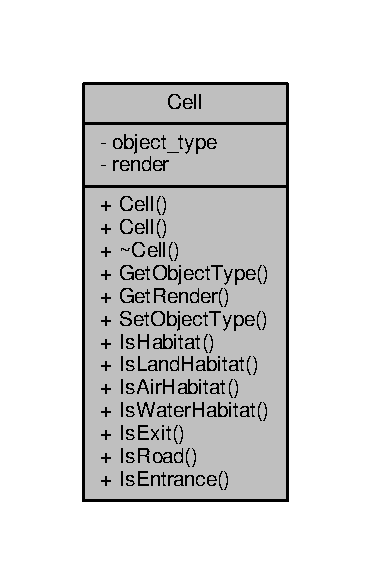
\includegraphics[width=178pt]{classCell__coll__graph}
\end{center}
\end{figure}
\subsection*{Classes}
\begin{DoxyCompactItemize}
\item 
class \hyperlink{classCell_1_1Kelas}{Kelas}
\end{DoxyCompactItemize}
\subsection*{Public Member Functions}
\begin{DoxyCompactItemize}
\item 
\hyperlink{classCell_a394510643e8664cf12b5efaf5cb99f71}{Cell} ()
\begin{DoxyCompactList}\small\item\em Constructor. Menciptakan \hyperlink{classCell}{Cell} kosong. \end{DoxyCompactList}\item 
\hyperlink{classCell_a26ca23bd35b1be145b8c161ac36b9bda}{Cell} (string ot)
\begin{DoxyCompactList}\small\item\em Constructor dengan parameter. Menciptakan \hyperlink{classCell}{Cell} kosong dengan tipe objek ot dan render r. \end{DoxyCompactList}\item 
\hyperlink{classCell_a9fa559f7a28e2b4336c6879ca09304d8}{$\sim$\+Cell} ()
\begin{DoxyCompactList}\small\item\em Destructor. \end{DoxyCompactList}\item 
string \hyperlink{classCell_a6218f05e1d9dcdf9ed61c5196040b1bd}{Get\+Object\+Type} () const 
\begin{DoxyCompactList}\small\item\em Getter untuk object type. \end{DoxyCompactList}\item 
char \hyperlink{classCell_a81e6357d206db3a6e6299029dc2273e5}{Get\+Render} () const 
\begin{DoxyCompactList}\small\item\em Getter untuk render. \end{DoxyCompactList}\item 
void \hyperlink{classCell_ad814dd782c42728917888c893b99b9df}{Set\+Object\+Type} (string ot)
\begin{DoxyCompactList}\small\item\em Setter untuk object type dari \hyperlink{classCell}{Cell}. \end{DoxyCompactList}\item 
bool \hyperlink{classCell_ab44ecb9c8347d20216b335af4e7c3700}{Is\+Habitat} ()
\begin{DoxyCompactList}\small\item\em Is\+Habitat. \end{DoxyCompactList}\item 
bool \hyperlink{classCell_a87c65d914c0be7928836fe8c46b5408e}{Is\+Land\+Habitat} ()
\begin{DoxyCompactList}\small\item\em Is\+Land\+Habitat. \end{DoxyCompactList}\item 
bool \hyperlink{classCell_af270b6bea6287714d585bae539edebc8}{Is\+Air\+Habitat} ()
\begin{DoxyCompactList}\small\item\em Is\+Air\+Habitat. \end{DoxyCompactList}\item 
bool \hyperlink{classCell_a06f065280a20d0008af9980ac4e053d0}{Is\+Water\+Habitat} ()
\begin{DoxyCompactList}\small\item\em Is\+Water\+Habitat. \end{DoxyCompactList}\item 
bool \hyperlink{classCell_a01c619a613088130f13c7d090121cbf5}{Is\+Exit} ()
\begin{DoxyCompactList}\small\item\em Is\+Exit. \end{DoxyCompactList}\item 
bool \hyperlink{classCell_aaaabb185d3c3d8ae23ac70dbc1148768}{Is\+Road} ()
\begin{DoxyCompactList}\small\item\em Is\+Road. \end{DoxyCompactList}\item 
bool \hyperlink{classCell_a15995ac65537db9e5bd3e6e1df7476e3}{Is\+Entrance} ()
\begin{DoxyCompactList}\small\item\em Is\+Entrance. \end{DoxyCompactList}\end{DoxyCompactItemize}
\subsection*{Private Attributes}
\begin{DoxyCompactItemize}
\item 
string \hyperlink{classCell_a800313ab2d6d6686a999e0179695737f}{object\+\_\+type}
\item 
char \hyperlink{classCell_a886f694017e919827f9208d17d3836d3}{render}
\end{DoxyCompactItemize}


\subsection{Constructor \& Destructor Documentation}
\index{Cell@{Cell}!Cell@{Cell}}
\index{Cell@{Cell}!Cell@{Cell}}
\subsubsection[{\texorpdfstring{Cell()}{Cell()}}]{\setlength{\rightskip}{0pt plus 5cm}Cell\+::\+Cell (
\begin{DoxyParamCaption}
{}
\end{DoxyParamCaption}
)}\hypertarget{classCell_a394510643e8664cf12b5efaf5cb99f71}{}\label{classCell_a394510643e8664cf12b5efaf5cb99f71}


Constructor. Menciptakan \hyperlink{classCell}{Cell} kosong. 

\index{Cell@{Cell}!Cell@{Cell}}
\index{Cell@{Cell}!Cell@{Cell}}
\subsubsection[{\texorpdfstring{Cell(string ot)}{Cell(string ot)}}]{\setlength{\rightskip}{0pt plus 5cm}Cell\+::\+Cell (
\begin{DoxyParamCaption}
\item[{string}]{ot}
\end{DoxyParamCaption}
)}\hypertarget{classCell_a26ca23bd35b1be145b8c161ac36b9bda}{}\label{classCell_a26ca23bd35b1be145b8c161ac36b9bda}


Constructor dengan parameter. Menciptakan \hyperlink{classCell}{Cell} kosong dengan tipe objek ot dan render r. 


\begin{DoxyParams}{Parameters}
{\em ot} & Object type dari \hyperlink{classCell}{Cell}. \\
\hline
{\em r} & Render dari \hyperlink{classCell}{Cell}. \\
\hline
\end{DoxyParams}
\index{Cell@{Cell}!````~Cell@{$\sim$\+Cell}}
\index{````~Cell@{$\sim$\+Cell}!Cell@{Cell}}
\subsubsection[{\texorpdfstring{$\sim$\+Cell()}{~Cell()}}]{\setlength{\rightskip}{0pt plus 5cm}Cell\+::$\sim$\+Cell (
\begin{DoxyParamCaption}
{}
\end{DoxyParamCaption}
)}\hypertarget{classCell_a9fa559f7a28e2b4336c6879ca09304d8}{}\label{classCell_a9fa559f7a28e2b4336c6879ca09304d8}


Destructor. 



\subsection{Member Function Documentation}
\index{Cell@{Cell}!Get\+Object\+Type@{Get\+Object\+Type}}
\index{Get\+Object\+Type@{Get\+Object\+Type}!Cell@{Cell}}
\subsubsection[{\texorpdfstring{Get\+Object\+Type() const }{GetObjectType() const }}]{\setlength{\rightskip}{0pt plus 5cm}string Cell\+::\+Get\+Object\+Type (
\begin{DoxyParamCaption}
{}
\end{DoxyParamCaption}
) const}\hypertarget{classCell_a6218f05e1d9dcdf9ed61c5196040b1bd}{}\label{classCell_a6218f05e1d9dcdf9ed61c5196040b1bd}


Getter untuk object type. 

\begin{DoxyReturn}{Returns}
Mengembalikan object type dari \hyperlink{classCell}{Cell}. 
\end{DoxyReturn}
\index{Cell@{Cell}!Get\+Render@{Get\+Render}}
\index{Get\+Render@{Get\+Render}!Cell@{Cell}}
\subsubsection[{\texorpdfstring{Get\+Render() const }{GetRender() const }}]{\setlength{\rightskip}{0pt plus 5cm}char Cell\+::\+Get\+Render (
\begin{DoxyParamCaption}
{}
\end{DoxyParamCaption}
) const}\hypertarget{classCell_a81e6357d206db3a6e6299029dc2273e5}{}\label{classCell_a81e6357d206db3a6e6299029dc2273e5}


Getter untuk render. 

\begin{DoxyReturn}{Returns}
Mengembalikan render dari \hyperlink{classCell}{Cell}. 
\end{DoxyReturn}
\index{Cell@{Cell}!Is\+Air\+Habitat@{Is\+Air\+Habitat}}
\index{Is\+Air\+Habitat@{Is\+Air\+Habitat}!Cell@{Cell}}
\subsubsection[{\texorpdfstring{Is\+Air\+Habitat()}{IsAirHabitat()}}]{\setlength{\rightskip}{0pt plus 5cm}bool Cell\+::\+Is\+Air\+Habitat (
\begin{DoxyParamCaption}
{}
\end{DoxyParamCaption}
)}\hypertarget{classCell_af270b6bea6287714d585bae539edebc8}{}\label{classCell_af270b6bea6287714d585bae539edebc8}


Is\+Air\+Habitat. 

\begin{DoxyReturn}{Returns}
Menghasilkan true jika code pada layar merupakan kode Air Habitat. 
\end{DoxyReturn}
\index{Cell@{Cell}!Is\+Entrance@{Is\+Entrance}}
\index{Is\+Entrance@{Is\+Entrance}!Cell@{Cell}}
\subsubsection[{\texorpdfstring{Is\+Entrance()}{IsEntrance()}}]{\setlength{\rightskip}{0pt plus 5cm}bool Cell\+::\+Is\+Entrance (
\begin{DoxyParamCaption}
{}
\end{DoxyParamCaption}
)}\hypertarget{classCell_a15995ac65537db9e5bd3e6e1df7476e3}{}\label{classCell_a15995ac65537db9e5bd3e6e1df7476e3}


Is\+Entrance. 

\begin{DoxyReturn}{Returns}
Menghasilkan true jika code pada layar merupakan kode Entrance. 
\end{DoxyReturn}
\index{Cell@{Cell}!Is\+Exit@{Is\+Exit}}
\index{Is\+Exit@{Is\+Exit}!Cell@{Cell}}
\subsubsection[{\texorpdfstring{Is\+Exit()}{IsExit()}}]{\setlength{\rightskip}{0pt plus 5cm}bool Cell\+::\+Is\+Exit (
\begin{DoxyParamCaption}
{}
\end{DoxyParamCaption}
)}\hypertarget{classCell_a01c619a613088130f13c7d090121cbf5}{}\label{classCell_a01c619a613088130f13c7d090121cbf5}


Is\+Exit. 

\begin{DoxyReturn}{Returns}
Menghasilkan true jika code pada layar merupakan kode Exit. 
\end{DoxyReturn}
\index{Cell@{Cell}!Is\+Habitat@{Is\+Habitat}}
\index{Is\+Habitat@{Is\+Habitat}!Cell@{Cell}}
\subsubsection[{\texorpdfstring{Is\+Habitat()}{IsHabitat()}}]{\setlength{\rightskip}{0pt plus 5cm}bool Cell\+::\+Is\+Habitat (
\begin{DoxyParamCaption}
{}
\end{DoxyParamCaption}
)}\hypertarget{classCell_ab44ecb9c8347d20216b335af4e7c3700}{}\label{classCell_ab44ecb9c8347d20216b335af4e7c3700}


Is\+Habitat. 

\begin{DoxyReturn}{Returns}
Menghasilkan true jika code pada layar merupakan kode Land, Air, atau Water Habitat. 
\end{DoxyReturn}
\index{Cell@{Cell}!Is\+Land\+Habitat@{Is\+Land\+Habitat}}
\index{Is\+Land\+Habitat@{Is\+Land\+Habitat}!Cell@{Cell}}
\subsubsection[{\texorpdfstring{Is\+Land\+Habitat()}{IsLandHabitat()}}]{\setlength{\rightskip}{0pt plus 5cm}bool Cell\+::\+Is\+Land\+Habitat (
\begin{DoxyParamCaption}
{}
\end{DoxyParamCaption}
)}\hypertarget{classCell_a87c65d914c0be7928836fe8c46b5408e}{}\label{classCell_a87c65d914c0be7928836fe8c46b5408e}


Is\+Land\+Habitat. 

\begin{DoxyReturn}{Returns}
Menghasilkan true jika code pada layar merupakan kode Land Habitat. 
\end{DoxyReturn}
\index{Cell@{Cell}!Is\+Road@{Is\+Road}}
\index{Is\+Road@{Is\+Road}!Cell@{Cell}}
\subsubsection[{\texorpdfstring{Is\+Road()}{IsRoad()}}]{\setlength{\rightskip}{0pt plus 5cm}bool Cell\+::\+Is\+Road (
\begin{DoxyParamCaption}
{}
\end{DoxyParamCaption}
)}\hypertarget{classCell_aaaabb185d3c3d8ae23ac70dbc1148768}{}\label{classCell_aaaabb185d3c3d8ae23ac70dbc1148768}


Is\+Road. 

\begin{DoxyReturn}{Returns}
Menghasilkan true jika code pada layar merupakan kode Road. 
\end{DoxyReturn}
\index{Cell@{Cell}!Is\+Water\+Habitat@{Is\+Water\+Habitat}}
\index{Is\+Water\+Habitat@{Is\+Water\+Habitat}!Cell@{Cell}}
\subsubsection[{\texorpdfstring{Is\+Water\+Habitat()}{IsWaterHabitat()}}]{\setlength{\rightskip}{0pt plus 5cm}bool Cell\+::\+Is\+Water\+Habitat (
\begin{DoxyParamCaption}
{}
\end{DoxyParamCaption}
)}\hypertarget{classCell_a06f065280a20d0008af9980ac4e053d0}{}\label{classCell_a06f065280a20d0008af9980ac4e053d0}


Is\+Water\+Habitat. 

\begin{DoxyReturn}{Returns}
Menghasilkan true jika code pada layar merupakan kode Water Habitat. 
\end{DoxyReturn}
\index{Cell@{Cell}!Set\+Object\+Type@{Set\+Object\+Type}}
\index{Set\+Object\+Type@{Set\+Object\+Type}!Cell@{Cell}}
\subsubsection[{\texorpdfstring{Set\+Object\+Type(string ot)}{SetObjectType(string ot)}}]{\setlength{\rightskip}{0pt plus 5cm}void Cell\+::\+Set\+Object\+Type (
\begin{DoxyParamCaption}
\item[{string}]{ot}
\end{DoxyParamCaption}
)}\hypertarget{classCell_ad814dd782c42728917888c893b99b9df}{}\label{classCell_ad814dd782c42728917888c893b99b9df}


Setter untuk object type dari \hyperlink{classCell}{Cell}. 


\begin{DoxyParams}{Parameters}
{\em ot} & Nilai object type yang akan di-\/set pada \hyperlink{classCell}{Cell}. \\
\hline
\end{DoxyParams}


\subsection{Member Data Documentation}
\index{Cell@{Cell}!object\+\_\+type@{object\+\_\+type}}
\index{object\+\_\+type@{object\+\_\+type}!Cell@{Cell}}
\subsubsection[{\texorpdfstring{object\+\_\+type}{object_type}}]{\setlength{\rightskip}{0pt plus 5cm}string Cell\+::object\+\_\+type\hspace{0.3cm}{\ttfamily [private]}}\hypertarget{classCell_a800313ab2d6d6686a999e0179695737f}{}\label{classCell_a800313ab2d6d6686a999e0179695737f}
\index{Cell@{Cell}!render@{render}}
\index{render@{render}!Cell@{Cell}}
\subsubsection[{\texorpdfstring{render}{render}}]{\setlength{\rightskip}{0pt plus 5cm}char Cell\+::render\hspace{0.3cm}{\ttfamily [private]}}\hypertarget{classCell_a886f694017e919827f9208d17d3836d3}{}\label{classCell_a886f694017e919827f9208d17d3836d3}


The documentation for this class was generated from the following files\+:\begin{DoxyCompactItemize}
\item 
cell/\hyperlink{cell_8h}{cell.\+h}\item 
cell/\hyperlink{cell_8cpp}{cell.\+cpp}\end{DoxyCompactItemize}

\hypertarget{classDriver}{}\section{Driver Class Reference}
\label{classDriver}\index{Driver@{Driver}}


{\ttfamily \#include $<$driver.\+h$>$}



Collaboration diagram for Driver\+:
\nopagebreak
\begin{figure}[H]
\begin{center}
\leavevmode
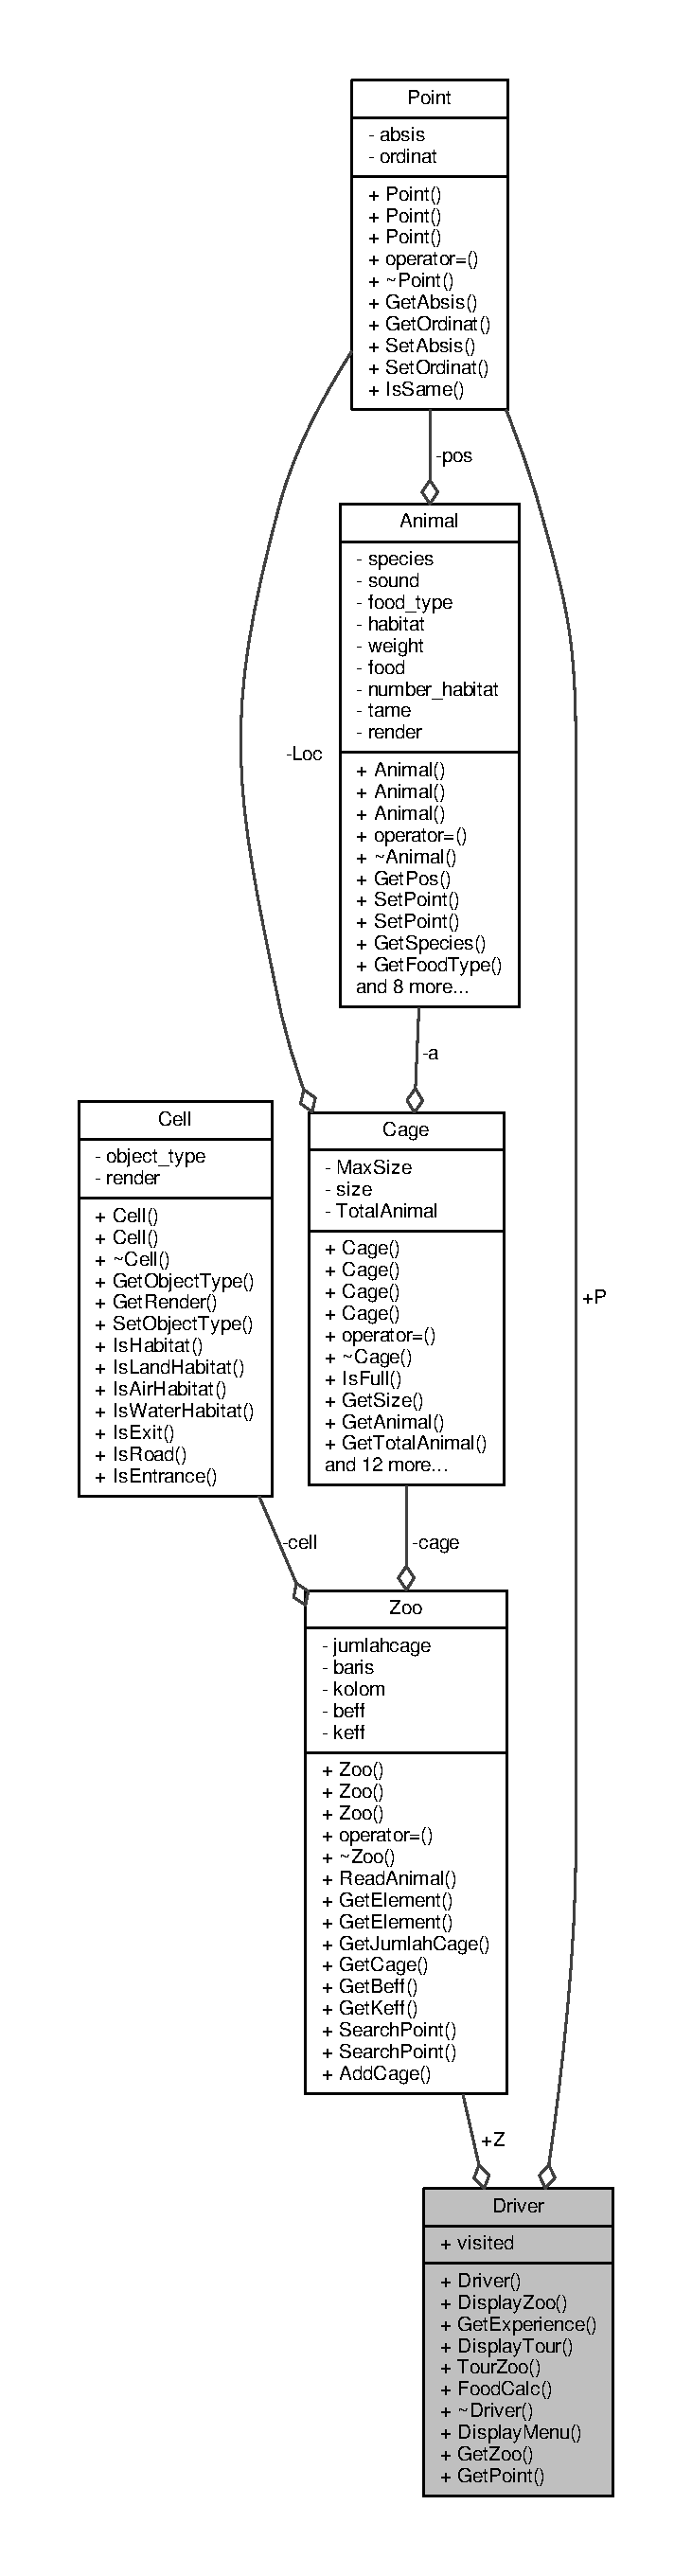
\includegraphics[height=550pt]{classDriver__coll__graph}
\end{center}
\end{figure}
\subsection*{Classes}
\begin{DoxyCompactItemize}
\item 
class \hyperlink{classDriver_1_1Kelas}{Kelas}
\end{DoxyCompactItemize}
\subsection*{Public Member Functions}
\begin{DoxyCompactItemize}
\item 
\hyperlink{classDriver_af0658d103e3e810a8e9ef0a53bb2e261}{Driver} ()
\begin{DoxyCompactList}\small\item\em Constructor. Menciptakan \hyperlink{classCage}{Cage} kosong tanpa animal. \end{DoxyCompactList}\item 
void \hyperlink{classDriver_aa8b4e139b99aad4720ce86286783dcdb}{Display\+Zoo} ()
\begin{DoxyCompactList}\small\item\em Display\+Zoo. Menampilkan zoo ke layar. \end{DoxyCompactList}\item 
void \hyperlink{classDriver_a2bc17a8251eab4cfdb7d74c7f7299c6e}{Get\+Experience} ()
\begin{DoxyCompactList}\small\item\em Get\+Experience. Mencetak ke layar eksperimen yang didapat pengunjung. \end{DoxyCompactList}\item 
void \hyperlink{classDriver_af3677b3b6adc2ccc5d486be1e4462fba}{Display\+Tour} ()
\begin{DoxyCompactList}\small\item\em Display\+Zoo. Menampilkan tur yang terjadi ke layar. \end{DoxyCompactList}\item 
void \hyperlink{classDriver_aa56ed0eaa789f78765708e15032d6534}{Tour\+Zoo} ()
\begin{DoxyCompactList}\small\item\em Tour\+Zoo. Melakukan tur zoo. \end{DoxyCompactList}\item 
float \hyperlink{classDriver_a0f85e40efd4983b0434307ca0647f378}{Food\+Calc} ()
\begin{DoxyCompactList}\small\item\em Food\+Calc. Melakukan perhitungan makanan yang harus disiapkan. \end{DoxyCompactList}\item 
\hyperlink{classDriver_ac7645eea8d3ce2bc39ddbda5e840297a}{$\sim$\+Driver} ()
\begin{DoxyCompactList}\small\item\em Destructor. \end{DoxyCompactList}\item 
void \hyperlink{classDriver_a56f5ca7386659854399999ffb6d8d043}{Display\+Menu} ()
\begin{DoxyCompactList}\small\item\em Display\+Menu. Menampilkan menu utama ke layar. \end{DoxyCompactList}\item 
\hyperlink{classZoo}{Zoo} \& \hyperlink{classDriver_a61680a5ffa5a314e4cb411b7bff29f26}{Get\+Zoo} ()
\begin{DoxyCompactList}\small\item\em Get\+Zoo. \end{DoxyCompactList}\item 
\hyperlink{classPoint}{Point} \& \hyperlink{classDriver_a5efd12ebb8faa45d7c95a23ed83ac5d5}{Get\+Point} ()
\begin{DoxyCompactList}\small\item\em Get\+Zoo. \end{DoxyCompactList}\end{DoxyCompactItemize}
\subsection*{Public Attributes}
\begin{DoxyCompactItemize}
\item 
\hyperlink{classZoo}{Zoo} \hyperlink{classDriver_a15f54a382cba3cdcf82c396cecfa3f9e}{Z}
\item 
bool $\ast$$\ast$ \hyperlink{classDriver_ab338d327140ab7a1a9469d5c16c2697f}{visited}
\item 
\hyperlink{classPoint}{Point} \hyperlink{classDriver_a967bca94eece374e66e7ed827f22cf51}{P}
\end{DoxyCompactItemize}


\subsection{Constructor \& Destructor Documentation}
\index{Driver@{Driver}!Driver@{Driver}}
\index{Driver@{Driver}!Driver@{Driver}}
\subsubsection[{\texorpdfstring{Driver()}{Driver()}}]{\setlength{\rightskip}{0pt plus 5cm}Driver\+::\+Driver (
\begin{DoxyParamCaption}
{}
\end{DoxyParamCaption}
)}\hypertarget{classDriver_af0658d103e3e810a8e9ef0a53bb2e261}{}\label{classDriver_af0658d103e3e810a8e9ef0a53bb2e261}


Constructor. Menciptakan \hyperlink{classCage}{Cage} kosong tanpa animal. 

\index{Driver@{Driver}!````~Driver@{$\sim$\+Driver}}
\index{````~Driver@{$\sim$\+Driver}!Driver@{Driver}}
\subsubsection[{\texorpdfstring{$\sim$\+Driver()}{~Driver()}}]{\setlength{\rightskip}{0pt plus 5cm}Driver\+::$\sim$\+Driver (
\begin{DoxyParamCaption}
{}
\end{DoxyParamCaption}
)\hspace{0.3cm}{\ttfamily [inline]}}\hypertarget{classDriver_ac7645eea8d3ce2bc39ddbda5e840297a}{}\label{classDriver_ac7645eea8d3ce2bc39ddbda5e840297a}


Destructor. 



\subsection{Member Function Documentation}
\index{Driver@{Driver}!Display\+Menu@{Display\+Menu}}
\index{Display\+Menu@{Display\+Menu}!Driver@{Driver}}
\subsubsection[{\texorpdfstring{Display\+Menu()}{DisplayMenu()}}]{\setlength{\rightskip}{0pt plus 5cm}void Driver\+::\+Display\+Menu (
\begin{DoxyParamCaption}
{}
\end{DoxyParamCaption}
)}\hypertarget{classDriver_a56f5ca7386659854399999ffb6d8d043}{}\label{classDriver_a56f5ca7386659854399999ffb6d8d043}


Display\+Menu. Menampilkan menu utama ke layar. 

\index{Driver@{Driver}!Display\+Tour@{Display\+Tour}}
\index{Display\+Tour@{Display\+Tour}!Driver@{Driver}}
\subsubsection[{\texorpdfstring{Display\+Tour()}{DisplayTour()}}]{\setlength{\rightskip}{0pt plus 5cm}void Driver\+::\+Display\+Tour (
\begin{DoxyParamCaption}
{}
\end{DoxyParamCaption}
)}\hypertarget{classDriver_af3677b3b6adc2ccc5d486be1e4462fba}{}\label{classDriver_af3677b3b6adc2ccc5d486be1e4462fba}


Display\+Zoo. Menampilkan tur yang terjadi ke layar. 

\index{Driver@{Driver}!Display\+Zoo@{Display\+Zoo}}
\index{Display\+Zoo@{Display\+Zoo}!Driver@{Driver}}
\subsubsection[{\texorpdfstring{Display\+Zoo()}{DisplayZoo()}}]{\setlength{\rightskip}{0pt plus 5cm}void Driver\+::\+Display\+Zoo (
\begin{DoxyParamCaption}
{}
\end{DoxyParamCaption}
)}\hypertarget{classDriver_aa8b4e139b99aad4720ce86286783dcdb}{}\label{classDriver_aa8b4e139b99aad4720ce86286783dcdb}


Display\+Zoo. Menampilkan zoo ke layar. 

\index{Driver@{Driver}!Food\+Calc@{Food\+Calc}}
\index{Food\+Calc@{Food\+Calc}!Driver@{Driver}}
\subsubsection[{\texorpdfstring{Food\+Calc()}{FoodCalc()}}]{\setlength{\rightskip}{0pt plus 5cm}float Driver\+::\+Food\+Calc (
\begin{DoxyParamCaption}
{}
\end{DoxyParamCaption}
)}\hypertarget{classDriver_a0f85e40efd4983b0434307ca0647f378}{}\label{classDriver_a0f85e40efd4983b0434307ca0647f378}


Food\+Calc. Melakukan perhitungan makanan yang harus disiapkan. 

\begin{DoxyReturn}{Returns}
Mengembalikan jumlah makanan yang harus disiapkan. 
\end{DoxyReturn}
\index{Driver@{Driver}!Get\+Experience@{Get\+Experience}}
\index{Get\+Experience@{Get\+Experience}!Driver@{Driver}}
\subsubsection[{\texorpdfstring{Get\+Experience()}{GetExperience()}}]{\setlength{\rightskip}{0pt plus 5cm}void Driver\+::\+Get\+Experience (
\begin{DoxyParamCaption}
{}
\end{DoxyParamCaption}
)}\hypertarget{classDriver_a2bc17a8251eab4cfdb7d74c7f7299c6e}{}\label{classDriver_a2bc17a8251eab4cfdb7d74c7f7299c6e}


Get\+Experience. Mencetak ke layar eksperimen yang didapat pengunjung. 

\index{Driver@{Driver}!Get\+Point@{Get\+Point}}
\index{Get\+Point@{Get\+Point}!Driver@{Driver}}
\subsubsection[{\texorpdfstring{Get\+Point()}{GetPoint()}}]{\setlength{\rightskip}{0pt plus 5cm}{\bf Point} \& Driver\+::\+Get\+Point (
\begin{DoxyParamCaption}
{}
\end{DoxyParamCaption}
)}\hypertarget{classDriver_a5efd12ebb8faa45d7c95a23ed83ac5d5}{}\label{classDriver_a5efd12ebb8faa45d7c95a23ed83ac5d5}


Get\+Zoo. 

\begin{DoxyReturn}{Returns}
Mengembalikan point. 
\end{DoxyReturn}
\index{Driver@{Driver}!Get\+Zoo@{Get\+Zoo}}
\index{Get\+Zoo@{Get\+Zoo}!Driver@{Driver}}
\subsubsection[{\texorpdfstring{Get\+Zoo()}{GetZoo()}}]{\setlength{\rightskip}{0pt plus 5cm}{\bf Zoo} \& Driver\+::\+Get\+Zoo (
\begin{DoxyParamCaption}
{}
\end{DoxyParamCaption}
)}\hypertarget{classDriver_a61680a5ffa5a314e4cb411b7bff29f26}{}\label{classDriver_a61680a5ffa5a314e4cb411b7bff29f26}


Get\+Zoo. 

\begin{DoxyReturn}{Returns}
Mengembalikan zoo. 
\end{DoxyReturn}
\index{Driver@{Driver}!Tour\+Zoo@{Tour\+Zoo}}
\index{Tour\+Zoo@{Tour\+Zoo}!Driver@{Driver}}
\subsubsection[{\texorpdfstring{Tour\+Zoo()}{TourZoo()}}]{\setlength{\rightskip}{0pt plus 5cm}void Driver\+::\+Tour\+Zoo (
\begin{DoxyParamCaption}
{}
\end{DoxyParamCaption}
)}\hypertarget{classDriver_aa56ed0eaa789f78765708e15032d6534}{}\label{classDriver_aa56ed0eaa789f78765708e15032d6534}


Tour\+Zoo. Melakukan tur zoo. 



\subsection{Member Data Documentation}
\index{Driver@{Driver}!P@{P}}
\index{P@{P}!Driver@{Driver}}
\subsubsection[{\texorpdfstring{P}{P}}]{\setlength{\rightskip}{0pt plus 5cm}{\bf Point} Driver\+::P}\hypertarget{classDriver_a967bca94eece374e66e7ed827f22cf51}{}\label{classDriver_a967bca94eece374e66e7ed827f22cf51}
\index{Driver@{Driver}!visited@{visited}}
\index{visited@{visited}!Driver@{Driver}}
\subsubsection[{\texorpdfstring{visited}{visited}}]{\setlength{\rightskip}{0pt plus 5cm}bool$\ast$$\ast$ Driver\+::visited}\hypertarget{classDriver_ab338d327140ab7a1a9469d5c16c2697f}{}\label{classDriver_ab338d327140ab7a1a9469d5c16c2697f}
\index{Driver@{Driver}!Z@{Z}}
\index{Z@{Z}!Driver@{Driver}}
\subsubsection[{\texorpdfstring{Z}{Z}}]{\setlength{\rightskip}{0pt plus 5cm}{\bf Zoo} Driver\+::Z}\hypertarget{classDriver_a15f54a382cba3cdcf82c396cecfa3f9e}{}\label{classDriver_a15f54a382cba3cdcf82c396cecfa3f9e}


The documentation for this class was generated from the following files\+:\begin{DoxyCompactItemize}
\item 
driver/\hyperlink{driver_8h}{driver.\+h}\item 
driver/\hyperlink{driver_8cpp}{driver.\+cpp}\end{DoxyCompactItemize}

\hypertarget{classCage_1_1Kelas}{}\section{Cage\+:\+:Kelas Class Reference}
\label{classCage_1_1Kelas}\index{Cage\+::\+Kelas@{Cage\+::\+Kelas}}


Collaboration diagram for Cage\+:\+:Kelas\+:
% FIG 0


\subsection{Detailed Description}
himpunan \hyperlink{classCell}{Cell} yang bertipe sama. 

The documentation for this class was generated from the following file\+:\begin{DoxyCompactItemize}
\item 
cage/\hyperlink{cage_8h}{cage.\+h}\end{DoxyCompactItemize}

\hypertarget{classDriver_1_1Kelas}{}\section{Driver\+:\+:Kelas Class Reference}
\label{classDriver_1_1Kelas}\index{Driver\+::\+Kelas@{Driver\+::\+Kelas}}


Collaboration diagram for Driver\+:\+:Kelas\+:
\nopagebreak
\begin{figure}[H]
\begin{center}
\leavevmode
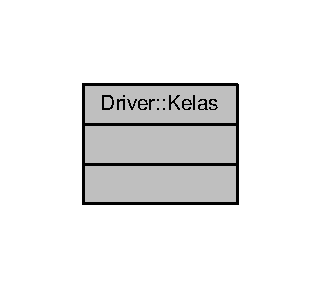
\includegraphics[width=154pt]{classDriver_1_1Kelas__coll__graph}
\end{center}
\end{figure}


\subsection{Detailed Description}
kelas sebagai pilihan menu aplikasi. 

The documentation for this class was generated from the following file\+:\begin{DoxyCompactItemize}
\item 
driver/\hyperlink{driver_8h}{driver.\+h}\end{DoxyCompactItemize}

\hypertarget{classCell_1_1Kelas}{}\section{Cell\+:\+:Kelas Class Reference}
\label{classCell_1_1Kelas}\index{Cell\+::\+Kelas@{Cell\+::\+Kelas}}


Collaboration diagram for Cell\+:\+:Kelas\+:\nopagebreak
\begin{figure}[H]
\begin{center}
\leavevmode
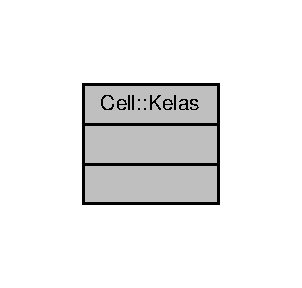
\includegraphics[width=145pt]{classCell_1_1Kelas__coll__graph}
\end{center}
\end{figure}


\subsection{Detailed Description}
simulasi dari petak-\/petak yang terdapat dalam kebun binatang. 

The documentation for this class was generated from the following file\+:\begin{DoxyCompactItemize}
\item 
cell/\hyperlink{cell_8h}{cell.\+h}\end{DoxyCompactItemize}

\hypertarget{classPoint}{}\section{Point Class Reference}
\label{classPoint}\index{Point@{Point}}


{\ttfamily \#include $<$point.\+h$>$}



Collaboration diagram for Point\+:
\nopagebreak
\begin{figure}[H]
\begin{center}
\leavevmode
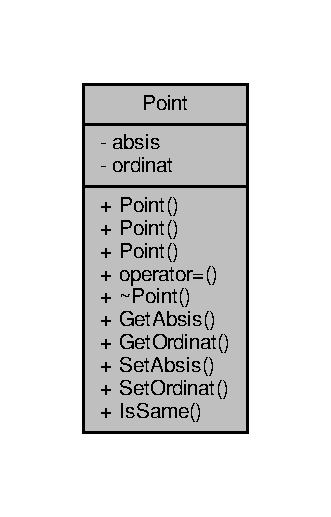
\includegraphics[width=159pt]{classPoint__coll__graph}
\end{center}
\end{figure}
\subsection*{Public Member Functions}
\begin{DoxyCompactItemize}
\item 
\hyperlink{classPoint_ad92f2337b839a94ce97dcdb439b4325a}{Point} ()
\begin{DoxyCompactList}\small\item\em Constructor. Menciptakan point kosong dengan absis dan ordinat sama dengan 0. \end{DoxyCompactList}\item 
\hyperlink{classPoint_a3634e1e4d94c1268ddaca3909f23b39b}{Point} (int abs, int ord)
\begin{DoxyCompactList}\small\item\em Constructor dengan parameter. Menciptakan point kosong dengan absis abs dan ordinat ord. \end{DoxyCompactList}\item 
\hyperlink{classPoint_a7e32c5a7f878c49ed9f1777b622cc06c}{Point} (const \hyperlink{classPoint}{Point} \&P)
\begin{DoxyCompactList}\small\item\em Copy Constructor. \end{DoxyCompactList}\item 
\hyperlink{classPoint}{Point} \& \hyperlink{classPoint_a24f658e4631df755120d856de77e3cbb}{operator=} (const \hyperlink{classPoint}{Point} \&P)
\begin{DoxyCompactList}\small\item\em Operator =. \end{DoxyCompactList}\item 
\hyperlink{classPoint_a395fa04b4ec126b66fc053f829a30cc1}{$\sim$\+Point} ()
\begin{DoxyCompactList}\small\item\em Destructor. \end{DoxyCompactList}\item 
int \hyperlink{classPoint_af9d064339ffb2f87abb6574dbfc9cdb2}{Get\+Absis} () const 
\begin{DoxyCompactList}\small\item\em Getter absis. \end{DoxyCompactList}\item 
int \hyperlink{classPoint_ace648a3faea60f8102d645d4b5a40b1a}{Get\+Ordinat} () const 
\begin{DoxyCompactList}\small\item\em Getter ordinat. \end{DoxyCompactList}\item 
void \hyperlink{classPoint_a0ba1dc33923b3aaa7678a07ffa022b06}{Set\+Absis} (int abs)
\begin{DoxyCompactList}\small\item\em Setter absis. \end{DoxyCompactList}\item 
void \hyperlink{classPoint_ae672d4952c6c730d104588a67304aed1}{Set\+Ordinat} (int ord)
\begin{DoxyCompactList}\small\item\em Setter ordinat. \end{DoxyCompactList}\item 
bool \hyperlink{classPoint_a19e146331c9acef35c6941bee733925e}{Is\+Same} (\hyperlink{classPoint}{Point} P) const 
\begin{DoxyCompactList}\small\item\em Memeriksa kesamaan dua point. \end{DoxyCompactList}\end{DoxyCompactItemize}


\subsection{Detailed Description}
Kelas \hyperlink{classPoint}{Point} merupakan kelas dengan atribut absis dan ordinat 

\subsection{Constructor \& Destructor Documentation}
\index{Point@{Point}!Point@{Point}}
\index{Point@{Point}!Point@{Point}}
\subsubsection[{\texorpdfstring{Point()}{Point()}}]{\setlength{\rightskip}{0pt plus 5cm}Point\+::\+Point (
\begin{DoxyParamCaption}
{}
\end{DoxyParamCaption}
)}\hypertarget{classPoint_ad92f2337b839a94ce97dcdb439b4325a}{}\label{classPoint_ad92f2337b839a94ce97dcdb439b4325a}


Constructor. Menciptakan point kosong dengan absis dan ordinat sama dengan 0. 

\index{Point@{Point}!Point@{Point}}
\index{Point@{Point}!Point@{Point}}
\subsubsection[{\texorpdfstring{Point(int abs, int ord)}{Point(int abs, int ord)}}]{\setlength{\rightskip}{0pt plus 5cm}Point\+::\+Point (
\begin{DoxyParamCaption}
\item[{int}]{abs, }
\item[{int}]{ord}
\end{DoxyParamCaption}
)}\hypertarget{classPoint_a3634e1e4d94c1268ddaca3909f23b39b}{}\label{classPoint_a3634e1e4d94c1268ddaca3909f23b39b}


Constructor dengan parameter. Menciptakan point kosong dengan absis abs dan ordinat ord. 


\begin{DoxyParams}{Parameters}
{\em abs} & Nilai absis point. \\
\hline
{\em ord} & Nilai ordinat point. \\
\hline
\end{DoxyParams}
\index{Point@{Point}!Point@{Point}}
\index{Point@{Point}!Point@{Point}}
\subsubsection[{\texorpdfstring{Point(const Point \&\+P)}{Point(const Point &P)}}]{\setlength{\rightskip}{0pt plus 5cm}Point\+::\+Point (
\begin{DoxyParamCaption}
\item[{const {\bf Point} \&}]{P}
\end{DoxyParamCaption}
)}\hypertarget{classPoint_a7e32c5a7f878c49ed9f1777b622cc06c}{}\label{classPoint_a7e32c5a7f878c49ed9f1777b622cc06c}


Copy Constructor. 


\begin{DoxyParams}{Parameters}
{\em P} & Objek yang akan di-\/copy. \\
\hline
\end{DoxyParams}
\index{Point@{Point}!````~Point@{$\sim$\+Point}}
\index{````~Point@{$\sim$\+Point}!Point@{Point}}
\subsubsection[{\texorpdfstring{$\sim$\+Point()}{~Point()}}]{\setlength{\rightskip}{0pt plus 5cm}Point\+::$\sim$\+Point (
\begin{DoxyParamCaption}
{}
\end{DoxyParamCaption}
)\hspace{0.3cm}{\ttfamily [inline]}}\hypertarget{classPoint_a395fa04b4ec126b66fc053f829a30cc1}{}\label{classPoint_a395fa04b4ec126b66fc053f829a30cc1}


Destructor. 



\subsection{Member Function Documentation}
\index{Point@{Point}!Get\+Absis@{Get\+Absis}}
\index{Get\+Absis@{Get\+Absis}!Point@{Point}}
\subsubsection[{\texorpdfstring{Get\+Absis() const }{GetAbsis() const }}]{\setlength{\rightskip}{0pt plus 5cm}int Point\+::\+Get\+Absis (
\begin{DoxyParamCaption}
{}
\end{DoxyParamCaption}
) const}\hypertarget{classPoint_af9d064339ffb2f87abb6574dbfc9cdb2}{}\label{classPoint_af9d064339ffb2f87abb6574dbfc9cdb2}


Getter absis. 

\begin{DoxyReturn}{Returns}
Mengembalikan nilai absis point. 
\end{DoxyReturn}
\index{Point@{Point}!Get\+Ordinat@{Get\+Ordinat}}
\index{Get\+Ordinat@{Get\+Ordinat}!Point@{Point}}
\subsubsection[{\texorpdfstring{Get\+Ordinat() const }{GetOrdinat() const }}]{\setlength{\rightskip}{0pt plus 5cm}int Point\+::\+Get\+Ordinat (
\begin{DoxyParamCaption}
{}
\end{DoxyParamCaption}
) const}\hypertarget{classPoint_ace648a3faea60f8102d645d4b5a40b1a}{}\label{classPoint_ace648a3faea60f8102d645d4b5a40b1a}


Getter ordinat. 

\begin{DoxyReturn}{Returns}
Mengembalikan nilai ordinat point. 
\end{DoxyReturn}
\index{Point@{Point}!Is\+Same@{Is\+Same}}
\index{Is\+Same@{Is\+Same}!Point@{Point}}
\subsubsection[{\texorpdfstring{Is\+Same(\+Point P) const }{IsSame(Point P) const }}]{\setlength{\rightskip}{0pt plus 5cm}bool Point\+::\+Is\+Same (
\begin{DoxyParamCaption}
\item[{{\bf Point}}]{P}
\end{DoxyParamCaption}
) const}\hypertarget{classPoint_a19e146331c9acef35c6941bee733925e}{}\label{classPoint_a19e146331c9acef35c6941bee733925e}


Memeriksa kesamaan dua point. 


\begin{DoxyParams}{Parameters}
{\em P} & Objek yang akan dibandingkan. \\
\hline
\end{DoxyParams}
\begin{DoxyReturn}{Returns}
Menghasilkan true jika P memiliki nilai yang sama dengan current object. 
\end{DoxyReturn}
\index{Point@{Point}!operator=@{operator=}}
\index{operator=@{operator=}!Point@{Point}}
\subsubsection[{\texorpdfstring{operator=(const Point \&\+P)}{operator=(const Point &P)}}]{\setlength{\rightskip}{0pt plus 5cm}{\bf Point} \& Point\+::operator= (
\begin{DoxyParamCaption}
\item[{const {\bf Point} \&}]{P}
\end{DoxyParamCaption}
)}\hypertarget{classPoint_a24f658e4631df755120d856de77e3cbb}{}\label{classPoint_a24f658e4631df755120d856de77e3cbb}


Operator =. 


\begin{DoxyParams}{Parameters}
{\em P} & Objek yang akan diassign. \\
\hline
\end{DoxyParams}
\begin{DoxyReturn}{Returns}
Menghasilkan objek hasil copy objek P. 
\end{DoxyReturn}
\index{Point@{Point}!Set\+Absis@{Set\+Absis}}
\index{Set\+Absis@{Set\+Absis}!Point@{Point}}
\subsubsection[{\texorpdfstring{Set\+Absis(int abs)}{SetAbsis(int abs)}}]{\setlength{\rightskip}{0pt plus 5cm}void Point\+::\+Set\+Absis (
\begin{DoxyParamCaption}
\item[{int}]{abs}
\end{DoxyParamCaption}
)}\hypertarget{classPoint_a0ba1dc33923b3aaa7678a07ffa022b06}{}\label{classPoint_a0ba1dc33923b3aaa7678a07ffa022b06}


Setter absis. 


\begin{DoxyParams}{Parameters}
{\em abs} & Nilai absis yang akan di-\/set pada point. \\
\hline
\end{DoxyParams}
\index{Point@{Point}!Set\+Ordinat@{Set\+Ordinat}}
\index{Set\+Ordinat@{Set\+Ordinat}!Point@{Point}}
\subsubsection[{\texorpdfstring{Set\+Ordinat(int ord)}{SetOrdinat(int ord)}}]{\setlength{\rightskip}{0pt plus 5cm}void Point\+::\+Set\+Ordinat (
\begin{DoxyParamCaption}
\item[{int}]{ord}
\end{DoxyParamCaption}
)}\hypertarget{classPoint_ae672d4952c6c730d104588a67304aed1}{}\label{classPoint_ae672d4952c6c730d104588a67304aed1}


Setter ordinat. 


\begin{DoxyParams}{Parameters}
{\em ord} & Nilai ord yang akan di-\/set pada point. \\
\hline
\end{DoxyParams}


The documentation for this class was generated from the following files\+:\begin{DoxyCompactItemize}
\item 
point/\hyperlink{point_8h}{point.\+h}\item 
point/\hyperlink{point_8cpp}{point.\+cpp}\end{DoxyCompactItemize}

\hypertarget{classZoo}{}\section{Zoo Class Reference}
\label{classZoo}\index{Zoo@{Zoo}}


{\ttfamily \#include $<$zoo.\+h$>$}



Collaboration diagram for Zoo\+:
\nopagebreak
\begin{figure}[H]
\begin{center}
\leavevmode
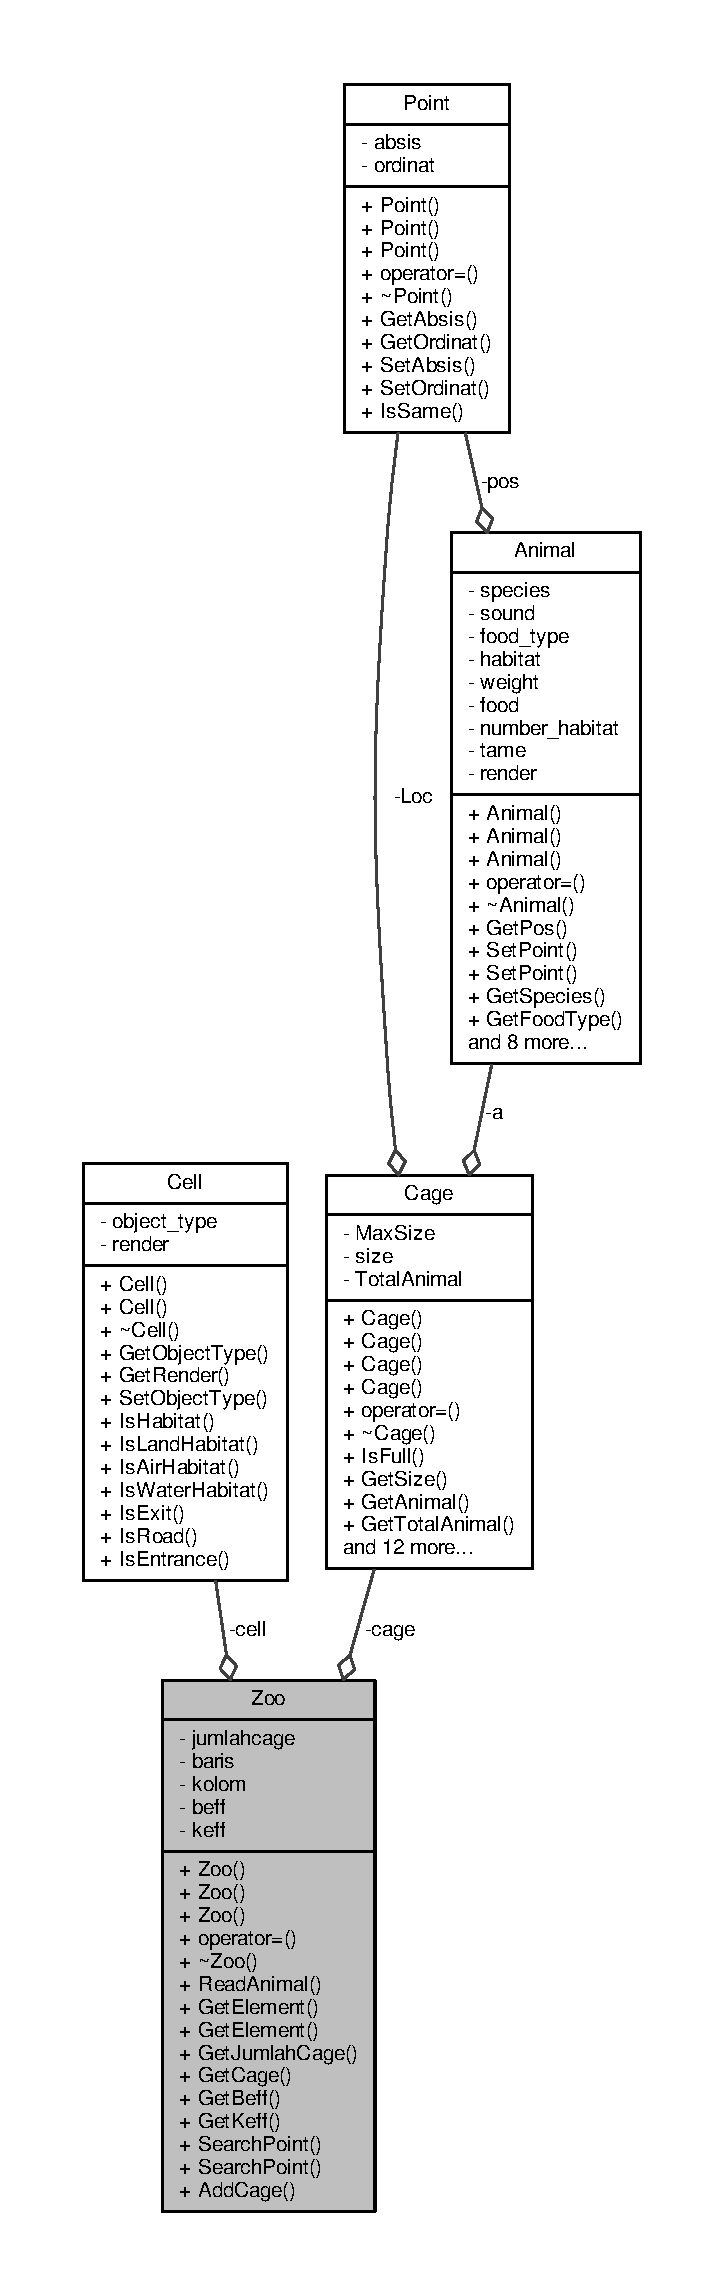
\includegraphics[height=550pt]{classZoo__coll__graph}
\end{center}
\end{figure}
\subsection*{Public Member Functions}
\begin{DoxyCompactItemize}
\item 
\hyperlink{classZoo_aaa0bf87b544fccd087e471ee0913709c}{Zoo} ()
\begin{DoxyCompactList}\small\item\em Constructor. Menciptakan zoo kosong yang berisi matriks kosong. \end{DoxyCompactList}\item 
\hyperlink{classZoo_a1d2ee3cc08057d114174ad997632f604}{Zoo} (int b, int k, int j)
\begin{DoxyCompactList}\small\item\em Constructor dengan parameter. Menciptakan zoo kosong dengan jumlah baris b, jumlah kolom k, dan jumlah cage j. \end{DoxyCompactList}\item 
\hyperlink{classZoo_a891edf2fa47d023068058e3745964e18}{Zoo} (const \hyperlink{classZoo}{Zoo} \&z)
\begin{DoxyCompactList}\small\item\em Copy Constructor. \end{DoxyCompactList}\item 
\hyperlink{classZoo}{Zoo} \& \hyperlink{classZoo_a62df0863e76f6d75a837c0445326deb7}{operator=} (const \hyperlink{classZoo}{Zoo} \&z)
\begin{DoxyCompactList}\small\item\em Operator =. \end{DoxyCompactList}\item 
\hyperlink{classZoo_ab65ebe1fa60f6cf2a7cc55f78ff06ba5}{$\sim$\+Zoo} ()
\begin{DoxyCompactList}\small\item\em Destrutor. \end{DoxyCompactList}\item 
void \hyperlink{classZoo_a56db9c646afb72b7d277b6bea76e675c}{Read\+Animal} ()
\begin{DoxyCompactList}\small\item\em Read\+Animal Membaca \hyperlink{classAnimal}{Animal} dari file eksternal. \end{DoxyCompactList}\item 
\hyperlink{classCell}{Cell} \& \hyperlink{classZoo_a0128c0b360793ac6aa8922b4cf2cc57f}{Get\+Element} (const \hyperlink{classPoint}{Point} \&P) const 
\begin{DoxyCompactList}\small\item\em Get\+Element. \end{DoxyCompactList}\item 
\hyperlink{classCell}{Cell} \& \hyperlink{classZoo_a5d21cf8cb0acdc6d4c9b625699a1d4a9}{Get\+Element} (int b, int k) const 
\begin{DoxyCompactList}\small\item\em Get\+Element. \end{DoxyCompactList}\item 
int \hyperlink{classZoo_ae0465354e9418560540b516b8563a590}{Get\+Jumlah\+Cage} () const 
\begin{DoxyCompactList}\small\item\em Get\+Jumlah\+Cage. \end{DoxyCompactList}\item 
\hyperlink{classCage}{Cage} \& \hyperlink{classZoo_a3956c403bc9f854aba57146896d264ea}{Get\+Cage} (int i) const 
\begin{DoxyCompactList}\small\item\em Get\+Cage. \end{DoxyCompactList}\item 
int \hyperlink{classZoo_a21590932eb500dd07226c1bbe2ce4726}{Get\+Beff} () const 
\begin{DoxyCompactList}\small\item\em Get\+Beff. \end{DoxyCompactList}\item 
int \hyperlink{classZoo_a759d40e997b024236da2a503662dca88}{Get\+Keff} () const 
\begin{DoxyCompactList}\small\item\em Get\+Keff. \end{DoxyCompactList}\item 
\hyperlink{classCage}{Cage} \& \hyperlink{classZoo_a99470f6b1415873b4e5f8cd25b2cf5a6}{Search\+Point} (const \hyperlink{classPoint}{Point} \&P) const 
\begin{DoxyCompactList}\small\item\em Search\+Point. Mencari point berada di cage mana. \end{DoxyCompactList}\item 
\hyperlink{classCage}{Cage} \& \hyperlink{classZoo_a8a984fb1f2c3b513cf986dec67c287bf}{Search\+Point} (int i, int j) const 
\begin{DoxyCompactList}\small\item\em Search\+Point. Mencari point berada di cage mana. \end{DoxyCompactList}\item 
void \hyperlink{classZoo_ad6095030bd48a8f51b4f83ff13fdf3b2}{Add\+Cage} (\hyperlink{classCage}{Cage} c)
\begin{DoxyCompactList}\small\item\em Add\+Cage. Menambahkan cage baru. \end{DoxyCompactList}\end{DoxyCompactItemize}
\subsection*{Private Attributes}
\begin{DoxyCompactItemize}
\item 
\hyperlink{classCell}{Cell} $\ast$$\ast$ \hyperlink{classZoo_a264dc6d031ca713ca28969120bb599ab}{cell}
\item 
\hyperlink{classCage}{Cage} $\ast$ \hyperlink{classZoo_a92269930ce6363c83b2b8fc7c8abd81d}{cage}
\item 
int \hyperlink{classZoo_ab9db4289e7ecd6856e4b7329dbde19d6}{jumlahcage}
\item 
const int \hyperlink{classZoo_a5aab4219fc1f6877609c6cd294abbc59}{baris}
\item 
const int \hyperlink{classZoo_a5ac40c8ba9d8a115c90c2aad733ee59c}{kolom}
\item 
int \hyperlink{classZoo_a859a09c6586ebfe53dc7504d0219e7cb}{beff}
\item 
int \hyperlink{classZoo_a9e90eb77a17d3767773b2a660d0ce981}{keff}
\end{DoxyCompactItemize}
\subsection*{Friends}
\begin{DoxyCompactItemize}
\item 
ostream \& \hyperlink{classZoo_a9a5a25ae9291345b74f5d8f7af9719db}{operator$<$$<$} (ostream \&o, const \hyperlink{classZoo}{Zoo} \&z)
\begin{DoxyCompactList}\small\item\em Operator $<$$<$. Melakukan print \hyperlink{classZoo}{Zoo}. \end{DoxyCompactList}\item 
istream \& \hyperlink{classZoo_a66565ea7c66ddb3acdcb0b67930b8615}{operator$>$$>$} (istream \&is, \hyperlink{classZoo}{Zoo} \&z)
\begin{DoxyCompactList}\small\item\em Operator $>$$>$. Melakukan read \hyperlink{classZoo}{Zoo}. \end{DoxyCompactList}\end{DoxyCompactItemize}


\subsection{Detailed Description}
Kelas \hyperlink{classZoo}{Zoo} merupakan simulasi dari kebun binatang berisi matriks \hyperlink{classCell}{Cell} 

\subsection{Constructor \& Destructor Documentation}
\index{Zoo@{Zoo}!Zoo@{Zoo}}
\index{Zoo@{Zoo}!Zoo@{Zoo}}
\subsubsection[{\texorpdfstring{Zoo()}{Zoo()}}]{\setlength{\rightskip}{0pt plus 5cm}Zoo\+::\+Zoo (
\begin{DoxyParamCaption}
{}
\end{DoxyParamCaption}
)}\hypertarget{classZoo_aaa0bf87b544fccd087e471ee0913709c}{}\label{classZoo_aaa0bf87b544fccd087e471ee0913709c}


Constructor. Menciptakan zoo kosong yang berisi matriks kosong. 

\index{Zoo@{Zoo}!Zoo@{Zoo}}
\index{Zoo@{Zoo}!Zoo@{Zoo}}
\subsubsection[{\texorpdfstring{Zoo(int b, int k, int j)}{Zoo(int b, int k, int j)}}]{\setlength{\rightskip}{0pt plus 5cm}Zoo\+::\+Zoo (
\begin{DoxyParamCaption}
\item[{int}]{b, }
\item[{int}]{k, }
\item[{int}]{j}
\end{DoxyParamCaption}
)}\hypertarget{classZoo_a1d2ee3cc08057d114174ad997632f604}{}\label{classZoo_a1d2ee3cc08057d114174ad997632f604}


Constructor dengan parameter. Menciptakan zoo kosong dengan jumlah baris b, jumlah kolom k, dan jumlah cage j. 


\begin{DoxyParams}{Parameters}
{\em b} & Nilai ukuran baris matriks. \\
\hline
{\em k} & Nilai ukuran kolom matriks. \\
\hline
{\em j} & Nilai banyaknya cage. \\
\hline
\end{DoxyParams}
\index{Zoo@{Zoo}!Zoo@{Zoo}}
\index{Zoo@{Zoo}!Zoo@{Zoo}}
\subsubsection[{\texorpdfstring{Zoo(const Zoo \&z)}{Zoo(const Zoo &z)}}]{\setlength{\rightskip}{0pt plus 5cm}Zoo\+::\+Zoo (
\begin{DoxyParamCaption}
\item[{const {\bf Zoo} \&}]{z}
\end{DoxyParamCaption}
)}\hypertarget{classZoo_a891edf2fa47d023068058e3745964e18}{}\label{classZoo_a891edf2fa47d023068058e3745964e18}


Copy Constructor. 


\begin{DoxyParams}{Parameters}
{\em z} & Objek yang akan di-\/copy. \\
\hline
\end{DoxyParams}
\index{Zoo@{Zoo}!````~Zoo@{$\sim$\+Zoo}}
\index{````~Zoo@{$\sim$\+Zoo}!Zoo@{Zoo}}
\subsubsection[{\texorpdfstring{$\sim$\+Zoo()}{~Zoo()}}]{\setlength{\rightskip}{0pt plus 5cm}Zoo\+::$\sim$\+Zoo (
\begin{DoxyParamCaption}
{}
\end{DoxyParamCaption}
)}\hypertarget{classZoo_ab65ebe1fa60f6cf2a7cc55f78ff06ba5}{}\label{classZoo_ab65ebe1fa60f6cf2a7cc55f78ff06ba5}


Destrutor. 



\subsection{Member Function Documentation}
\index{Zoo@{Zoo}!Add\+Cage@{Add\+Cage}}
\index{Add\+Cage@{Add\+Cage}!Zoo@{Zoo}}
\subsubsection[{\texorpdfstring{Add\+Cage(\+Cage c)}{AddCage(Cage c)}}]{\setlength{\rightskip}{0pt plus 5cm}void Zoo\+::\+Add\+Cage (
\begin{DoxyParamCaption}
\item[{{\bf Cage}}]{c}
\end{DoxyParamCaption}
)}\hypertarget{classZoo_ad6095030bd48a8f51b4f83ff13fdf3b2}{}\label{classZoo_ad6095030bd48a8f51b4f83ff13fdf3b2}


Add\+Cage. Menambahkan cage baru. 


\begin{DoxyParams}{Parameters}
{\em c} & \hyperlink{classCage}{Cage} yang ingin ditambahkan \\
\hline
\end{DoxyParams}
\index{Zoo@{Zoo}!Get\+Beff@{Get\+Beff}}
\index{Get\+Beff@{Get\+Beff}!Zoo@{Zoo}}
\subsubsection[{\texorpdfstring{Get\+Beff() const }{GetBeff() const }}]{\setlength{\rightskip}{0pt plus 5cm}int Zoo\+::\+Get\+Beff (
\begin{DoxyParamCaption}
{}
\end{DoxyParamCaption}
) const\hspace{0.3cm}{\ttfamily [inline]}}\hypertarget{classZoo_a21590932eb500dd07226c1bbe2ce4726}{}\label{classZoo_a21590932eb500dd07226c1bbe2ce4726}


Get\+Beff. 

\begin{DoxyReturn}{Returns}
Mengembalikan baris efektif zoo. 
\end{DoxyReturn}
\index{Zoo@{Zoo}!Get\+Cage@{Get\+Cage}}
\index{Get\+Cage@{Get\+Cage}!Zoo@{Zoo}}
\subsubsection[{\texorpdfstring{Get\+Cage(int i) const }{GetCage(int i) const }}]{\setlength{\rightskip}{0pt plus 5cm}{\bf Cage} \& Zoo\+::\+Get\+Cage (
\begin{DoxyParamCaption}
\item[{int}]{i}
\end{DoxyParamCaption}
) const}\hypertarget{classZoo_a3956c403bc9f854aba57146896d264ea}{}\label{classZoo_a3956c403bc9f854aba57146896d264ea}


Get\+Cage. 


\begin{DoxyParams}{Parameters}
{\em i} & Nilai indeks yang akan dikeluarkan cage nya. \\
\hline
\end{DoxyParams}
\begin{DoxyReturn}{Returns}
Mengembalikan cage zoo pada indeks ke-\/i. 
\end{DoxyReturn}
\index{Zoo@{Zoo}!Get\+Element@{Get\+Element}}
\index{Get\+Element@{Get\+Element}!Zoo@{Zoo}}
\subsubsection[{\texorpdfstring{Get\+Element(const Point \&\+P) const }{GetElement(const Point &P) const }}]{\setlength{\rightskip}{0pt plus 5cm}{\bf Cell} \& Zoo\+::\+Get\+Element (
\begin{DoxyParamCaption}
\item[{const {\bf Point} \&}]{P}
\end{DoxyParamCaption}
) const}\hypertarget{classZoo_a0128c0b360793ac6aa8922b4cf2cc57f}{}\label{classZoo_a0128c0b360793ac6aa8922b4cf2cc57f}


Get\+Element. 


\begin{DoxyParams}{Parameters}
{\em P} & \hyperlink{classPoint}{Point} yang akan diambil. \\
\hline
\end{DoxyParams}
\begin{DoxyReturn}{Returns}
Mengembalikan cell yang terdapat pada lokasi point P. 
\end{DoxyReturn}
\index{Zoo@{Zoo}!Get\+Element@{Get\+Element}}
\index{Get\+Element@{Get\+Element}!Zoo@{Zoo}}
\subsubsection[{\texorpdfstring{Get\+Element(int b, int k) const }{GetElement(int b, int k) const }}]{\setlength{\rightskip}{0pt plus 5cm}{\bf Cell} \& Zoo\+::\+Get\+Element (
\begin{DoxyParamCaption}
\item[{int}]{b, }
\item[{int}]{k}
\end{DoxyParamCaption}
) const}\hypertarget{classZoo_a5d21cf8cb0acdc6d4c9b625699a1d4a9}{}\label{classZoo_a5d21cf8cb0acdc6d4c9b625699a1d4a9}


Get\+Element. 


\begin{DoxyParams}{Parameters}
{\em b} & Nilai baris yang akan diambil. \\
\hline
{\em k} & Nilai kolom yang akan diambil. \\
\hline
\end{DoxyParams}
\begin{DoxyReturn}{Returns}
Mengembalikan cell yang terdapat pada baris ke b dan kolom ke k. 
\end{DoxyReturn}
\index{Zoo@{Zoo}!Get\+Jumlah\+Cage@{Get\+Jumlah\+Cage}}
\index{Get\+Jumlah\+Cage@{Get\+Jumlah\+Cage}!Zoo@{Zoo}}
\subsubsection[{\texorpdfstring{Get\+Jumlah\+Cage() const }{GetJumlahCage() const }}]{\setlength{\rightskip}{0pt plus 5cm}int Zoo\+::\+Get\+Jumlah\+Cage (
\begin{DoxyParamCaption}
{}
\end{DoxyParamCaption}
) const}\hypertarget{classZoo_ae0465354e9418560540b516b8563a590}{}\label{classZoo_ae0465354e9418560540b516b8563a590}


Get\+Jumlah\+Cage. 

\begin{DoxyReturn}{Returns}
Mengembalikan jumlah cage pada zoo. 
\end{DoxyReturn}
\index{Zoo@{Zoo}!Get\+Keff@{Get\+Keff}}
\index{Get\+Keff@{Get\+Keff}!Zoo@{Zoo}}
\subsubsection[{\texorpdfstring{Get\+Keff() const }{GetKeff() const }}]{\setlength{\rightskip}{0pt plus 5cm}int Zoo\+::\+Get\+Keff (
\begin{DoxyParamCaption}
{}
\end{DoxyParamCaption}
) const\hspace{0.3cm}{\ttfamily [inline]}}\hypertarget{classZoo_a759d40e997b024236da2a503662dca88}{}\label{classZoo_a759d40e997b024236da2a503662dca88}


Get\+Keff. 

\begin{DoxyReturn}{Returns}
Mengembalikan kolom efektif zoo. 
\end{DoxyReturn}
\index{Zoo@{Zoo}!operator=@{operator=}}
\index{operator=@{operator=}!Zoo@{Zoo}}
\subsubsection[{\texorpdfstring{operator=(const Zoo \&z)}{operator=(const Zoo &z)}}]{\setlength{\rightskip}{0pt plus 5cm}{\bf Zoo} \& Zoo\+::operator= (
\begin{DoxyParamCaption}
\item[{const {\bf Zoo} \&}]{z}
\end{DoxyParamCaption}
)}\hypertarget{classZoo_a62df0863e76f6d75a837c0445326deb7}{}\label{classZoo_a62df0863e76f6d75a837c0445326deb7}


Operator =. 


\begin{DoxyParams}{Parameters}
{\em z} & Objek yang akan di-\/assign. \\
\hline
\end{DoxyParams}
\begin{DoxyReturn}{Returns}
Menghasilkan objek hasil copy objek z. 
\end{DoxyReturn}
\index{Zoo@{Zoo}!Read\+Animal@{Read\+Animal}}
\index{Read\+Animal@{Read\+Animal}!Zoo@{Zoo}}
\subsubsection[{\texorpdfstring{Read\+Animal()}{ReadAnimal()}}]{\setlength{\rightskip}{0pt plus 5cm}void Zoo\+::\+Read\+Animal (
\begin{DoxyParamCaption}
{}
\end{DoxyParamCaption}
)}\hypertarget{classZoo_a56db9c646afb72b7d277b6bea76e675c}{}\label{classZoo_a56db9c646afb72b7d277b6bea76e675c}


Read\+Animal Membaca \hyperlink{classAnimal}{Animal} dari file eksternal. 

\index{Zoo@{Zoo}!Search\+Point@{Search\+Point}}
\index{Search\+Point@{Search\+Point}!Zoo@{Zoo}}
\subsubsection[{\texorpdfstring{Search\+Point(const Point \&\+P) const }{SearchPoint(const Point &P) const }}]{\setlength{\rightskip}{0pt plus 5cm}{\bf Cage} \& Zoo\+::\+Search\+Point (
\begin{DoxyParamCaption}
\item[{const {\bf Point} \&}]{P}
\end{DoxyParamCaption}
) const}\hypertarget{classZoo_a99470f6b1415873b4e5f8cd25b2cf5a6}{}\label{classZoo_a99470f6b1415873b4e5f8cd25b2cf5a6}


Search\+Point. Mencari point berada di cage mana. 


\begin{DoxyParams}{Parameters}
{\em P} & \hyperlink{classPoint}{Point} yang akan dicari. \\
\hline
\end{DoxyParams}
\begin{DoxyReturn}{Returns}
Mengeluarkan cage yang mengandung P. 
\end{DoxyReturn}
\index{Zoo@{Zoo}!Search\+Point@{Search\+Point}}
\index{Search\+Point@{Search\+Point}!Zoo@{Zoo}}
\subsubsection[{\texorpdfstring{Search\+Point(int i, int j) const }{SearchPoint(int i, int j) const }}]{\setlength{\rightskip}{0pt plus 5cm}{\bf Cage} \& Zoo\+::\+Search\+Point (
\begin{DoxyParamCaption}
\item[{int}]{i, }
\item[{int}]{j}
\end{DoxyParamCaption}
) const}\hypertarget{classZoo_a8a984fb1f2c3b513cf986dec67c287bf}{}\label{classZoo_a8a984fb1f2c3b513cf986dec67c287bf}


Search\+Point. Mencari point berada di cage mana. 


\begin{DoxyParams}{Parameters}
{\em i} & dan j absis dan ordinat yang akan dicari. \\
\hline
\end{DoxyParams}
\begin{DoxyReturn}{Returns}
Mengeluarkan cage yang mengandung P. 
\end{DoxyReturn}


\subsection{Friends And Related Function Documentation}
\index{Zoo@{Zoo}!operator$<$$<$@{operator$<$$<$}}
\index{operator$<$$<$@{operator$<$$<$}!Zoo@{Zoo}}
\subsubsection[{\texorpdfstring{operator$<$$<$}{operator<<}}]{\setlength{\rightskip}{0pt plus 5cm}ostream\& operator$<$$<$ (
\begin{DoxyParamCaption}
\item[{ostream \&}]{o, }
\item[{const {\bf Zoo} \&}]{z}
\end{DoxyParamCaption}
)\hspace{0.3cm}{\ttfamily [friend]}}\hypertarget{classZoo_a9a5a25ae9291345b74f5d8f7af9719db}{}\label{classZoo_a9a5a25ae9291345b74f5d8f7af9719db}


Operator $<$$<$. Melakukan print \hyperlink{classZoo}{Zoo}. 


\begin{DoxyParams}{Parameters}
{\em o} & Objek ostream. \\
\hline
{\em z} & Objek \hyperlink{classZoo}{Zoo} yang akan dicetak. \\
\hline
\end{DoxyParams}
\begin{DoxyReturn}{Returns}
Menghasilkan objek ostream yang akan dicetak. 
\end{DoxyReturn}
\index{Zoo@{Zoo}!operator$>$$>$@{operator$>$$>$}}
\index{operator$>$$>$@{operator$>$$>$}!Zoo@{Zoo}}
\subsubsection[{\texorpdfstring{operator$>$$>$}{operator>>}}]{\setlength{\rightskip}{0pt plus 5cm}istream\& operator$>$$>$ (
\begin{DoxyParamCaption}
\item[{istream \&}]{is, }
\item[{{\bf Zoo} \&}]{z}
\end{DoxyParamCaption}
)\hspace{0.3cm}{\ttfamily [friend]}}\hypertarget{classZoo_a66565ea7c66ddb3acdcb0b67930b8615}{}\label{classZoo_a66565ea7c66ddb3acdcb0b67930b8615}


Operator $>$$>$. Melakukan read \hyperlink{classZoo}{Zoo}. 


\begin{DoxyParams}{Parameters}
{\em i} & Objek istream. \\
\hline
{\em z} & Objek \hyperlink{classZoo}{Zoo} yang akan dibaca. \\
\hline
\end{DoxyParams}
\begin{DoxyReturn}{Returns}
Mengeluarkan objek istream yang telah dibaca. 
\end{DoxyReturn}


\subsection{Member Data Documentation}
\index{Zoo@{Zoo}!baris@{baris}}
\index{baris@{baris}!Zoo@{Zoo}}
\subsubsection[{\texorpdfstring{baris}{baris}}]{\setlength{\rightskip}{0pt plus 5cm}const int Zoo\+::baris\hspace{0.3cm}{\ttfamily [private]}}\hypertarget{classZoo_a5aab4219fc1f6877609c6cd294abbc59}{}\label{classZoo_a5aab4219fc1f6877609c6cd294abbc59}
\index{Zoo@{Zoo}!beff@{beff}}
\index{beff@{beff}!Zoo@{Zoo}}
\subsubsection[{\texorpdfstring{beff}{beff}}]{\setlength{\rightskip}{0pt plus 5cm}int Zoo\+::beff\hspace{0.3cm}{\ttfamily [private]}}\hypertarget{classZoo_a859a09c6586ebfe53dc7504d0219e7cb}{}\label{classZoo_a859a09c6586ebfe53dc7504d0219e7cb}
\index{Zoo@{Zoo}!cage@{cage}}
\index{cage@{cage}!Zoo@{Zoo}}
\subsubsection[{\texorpdfstring{cage}{cage}}]{\setlength{\rightskip}{0pt plus 5cm}{\bf Cage}$\ast$ Zoo\+::cage\hspace{0.3cm}{\ttfamily [private]}}\hypertarget{classZoo_a92269930ce6363c83b2b8fc7c8abd81d}{}\label{classZoo_a92269930ce6363c83b2b8fc7c8abd81d}
\index{Zoo@{Zoo}!cell@{cell}}
\index{cell@{cell}!Zoo@{Zoo}}
\subsubsection[{\texorpdfstring{cell}{cell}}]{\setlength{\rightskip}{0pt plus 5cm}{\bf Cell}$\ast$$\ast$ Zoo\+::cell\hspace{0.3cm}{\ttfamily [private]}}\hypertarget{classZoo_a264dc6d031ca713ca28969120bb599ab}{}\label{classZoo_a264dc6d031ca713ca28969120bb599ab}
\index{Zoo@{Zoo}!jumlahcage@{jumlahcage}}
\index{jumlahcage@{jumlahcage}!Zoo@{Zoo}}
\subsubsection[{\texorpdfstring{jumlahcage}{jumlahcage}}]{\setlength{\rightskip}{0pt plus 5cm}int Zoo\+::jumlahcage\hspace{0.3cm}{\ttfamily [private]}}\hypertarget{classZoo_ab9db4289e7ecd6856e4b7329dbde19d6}{}\label{classZoo_ab9db4289e7ecd6856e4b7329dbde19d6}
\index{Zoo@{Zoo}!keff@{keff}}
\index{keff@{keff}!Zoo@{Zoo}}
\subsubsection[{\texorpdfstring{keff}{keff}}]{\setlength{\rightskip}{0pt plus 5cm}int Zoo\+::keff\hspace{0.3cm}{\ttfamily [private]}}\hypertarget{classZoo_a9e90eb77a17d3767773b2a660d0ce981}{}\label{classZoo_a9e90eb77a17d3767773b2a660d0ce981}
\index{Zoo@{Zoo}!kolom@{kolom}}
\index{kolom@{kolom}!Zoo@{Zoo}}
\subsubsection[{\texorpdfstring{kolom}{kolom}}]{\setlength{\rightskip}{0pt plus 5cm}const int Zoo\+::kolom\hspace{0.3cm}{\ttfamily [private]}}\hypertarget{classZoo_a5ac40c8ba9d8a115c90c2aad733ee59c}{}\label{classZoo_a5ac40c8ba9d8a115c90c2aad733ee59c}


The documentation for this class was generated from the following files\+:\begin{DoxyCompactItemize}
\item 
zoo/\hyperlink{zoo_8h}{zoo.\+h}\item 
zoo/\hyperlink{zoo_8cpp}{zoo.\+cpp}\end{DoxyCompactItemize}

\chapter{File Documentation}
\hypertarget{animal_8txt}{}\section{animal.\+txt File Reference}
\label{animal_8txt}\index{animal.\+txt@{animal.\+txt}}

\hypertarget{animal_8cpp}{}\section{animal.\+cpp File Reference}
\label{animal_8cpp}\index{animal.\+cpp@{animal.\+cpp}}
{\ttfamily \#include \char`\"{}animal.\+h\char`\"{}}\\*
Include dependency graph for animal.\+cpp\+:
\nopagebreak
\begin{figure}[H]
\begin{center}
\leavevmode
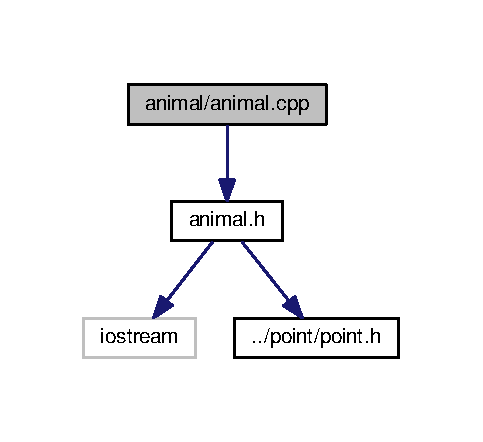
\includegraphics[width=198pt]{animal_8cpp__incl}
\end{center}
\end{figure}

\hypertarget{animal_8h}{}\section{animal.\+h File Reference}
\label{animal_8h}\index{animal.\+h@{animal.\+h}}
{\ttfamily \#include $<$iostream$>$}\\*
{\ttfamily \#include \char`\"{}point.\+h\char`\"{}}\\*
Include dependency graph for animal.\+h\+:
\nopagebreak
\begin{figure}[H]
\begin{center}
\leavevmode
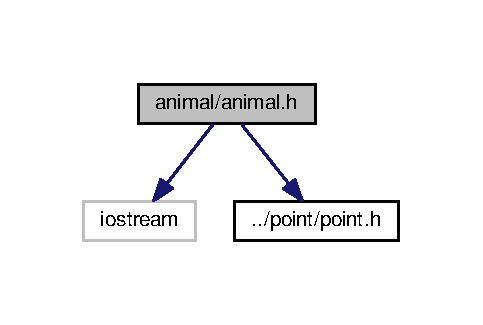
\includegraphics[width=198pt]{animal_8h__incl}
\end{center}
\end{figure}
This graph shows which files directly or indirectly include this file\+:
\nopagebreak
\begin{figure}[H]
\begin{center}
\leavevmode
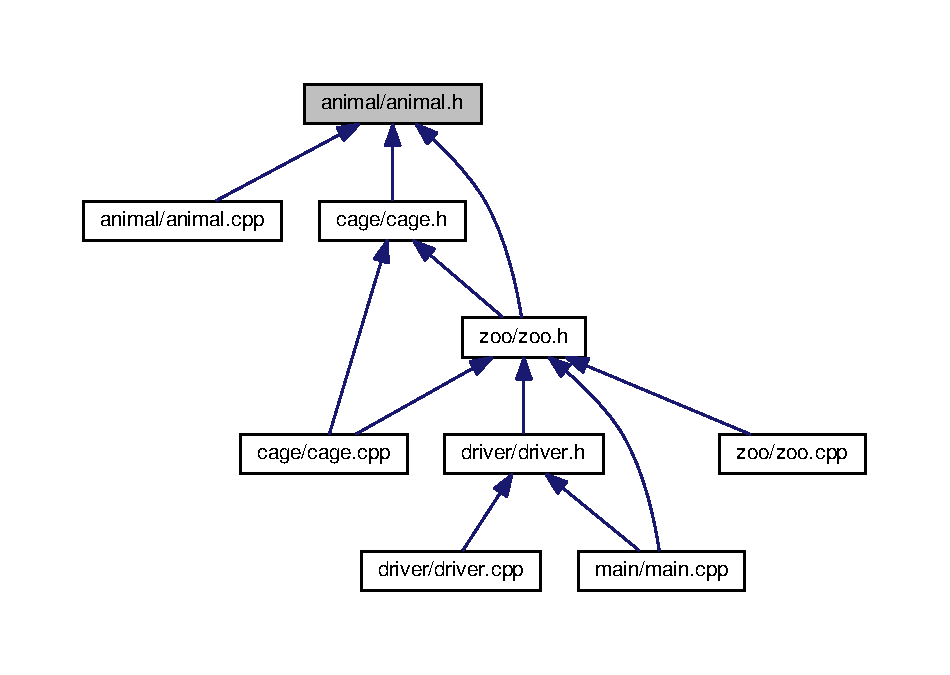
\includegraphics[width=350pt]{animal_8h__dep__incl}
\end{center}
\end{figure}
\subsection*{Classes}
\begin{DoxyCompactItemize}
\item 
class \hyperlink{classAnimal}{Animal}
\end{DoxyCompactItemize}

\hypertarget{cage_8cpp}{}\section{cage/cage.cpp File Reference}
\label{cage_8cpp}\index{cage/cage.\+cpp@{cage/cage.\+cpp}}
{\ttfamily \#include \char`\"{}cage.\+h\char`\"{}}\\*
{\ttfamily \#include \char`\"{}../zoo/zoo.\+h\char`\"{}}\\*
{\ttfamily \#include $<$iostream$>$}\\*
{\ttfamily \#include $<$cstdlib$>$}\\*
{\ttfamily \#include $<$ctime$>$}\\*
Include dependency graph for cage.\+cpp\+:
% FIG 0

\hypertarget{cage_8h}{}\section{cage/cage.h File Reference}
\label{cage_8h}\index{cage/cage.\+h@{cage/cage.\+h}}
{\ttfamily \#include \char`\"{}../point/point.\+h\char`\"{}}\\*
{\ttfamily \#include \char`\"{}../animal/animal.\+h\char`\"{}}\\*
Include dependency graph for cage.\+h\+:
% FIG 0
This graph shows which files directly or indirectly include this file\+:
% FIG 1
\subsection*{Classes}
\begin{DoxyCompactItemize}
\item 
class \hyperlink{classCage}{Cage}
\end{DoxyCompactItemize}

\hypertarget{cell_8cpp}{}\section{cell/cell.cpp File Reference}
\label{cell_8cpp}\index{cell/cell.\+cpp@{cell/cell.\+cpp}}
{\ttfamily \#include \char`\"{}cell.\+h\char`\"{}}\\*
Include dependency graph for cell.\+cpp\+:\nopagebreak
\begin{figure}[H]
\begin{center}
\leavevmode
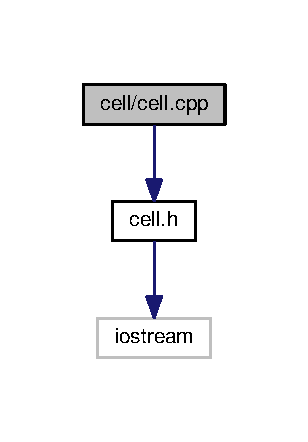
\includegraphics[width=148pt]{cell_8cpp__incl}
\end{center}
\end{figure}

\hypertarget{cell_8h}{}\section{cell/cell.h File Reference}
\label{cell_8h}\index{cell/cell.\+h@{cell/cell.\+h}}
{\ttfamily \#include $<$iostream$>$}\\*
Include dependency graph for cell.\+h\+:\nopagebreak
\begin{figure}[H]
\begin{center}
\leavevmode
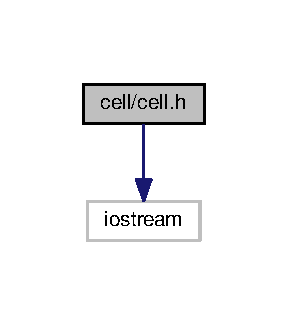
\includegraphics[width=138pt]{cell_8h__incl}
\end{center}
\end{figure}
This graph shows which files directly or indirectly include this file\+:\nopagebreak
\begin{figure}[H]
\begin{center}
\leavevmode
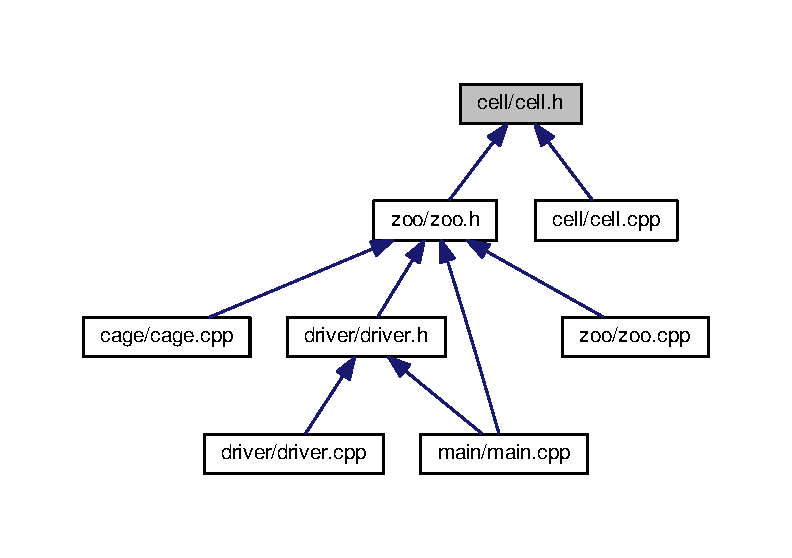
\includegraphics[width=350pt]{cell_8h__dep__incl}
\end{center}
\end{figure}
\subsection*{Classes}
\begin{DoxyCompactItemize}
\item 
class \hyperlink{classCell}{Cell}
\end{DoxyCompactItemize}

\hypertarget{driver_8cpp}{}\section{driver/driver.cpp File Reference}
\label{driver_8cpp}\index{driver/driver.\+cpp@{driver/driver.\+cpp}}
{\ttfamily \#include \char`\"{}driver.\+h\char`\"{}}\\*
{\ttfamily \#include $<$fstream$>$}\\*
{\ttfamily \#include $<$iostream$>$}\\*
Include dependency graph for driver.\+cpp\+:
% FIG 0

\hypertarget{driver_8h}{}\section{driver/driver.h File Reference}
\label{driver_8h}\index{driver/driver.\+h@{driver/driver.\+h}}
{\ttfamily \#include \char`\"{}../zoo/zoo.\+h\char`\"{}}\\*
Include dependency graph for driver.\+h\+:\nopagebreak
\begin{figure}[H]
\begin{center}
\leavevmode
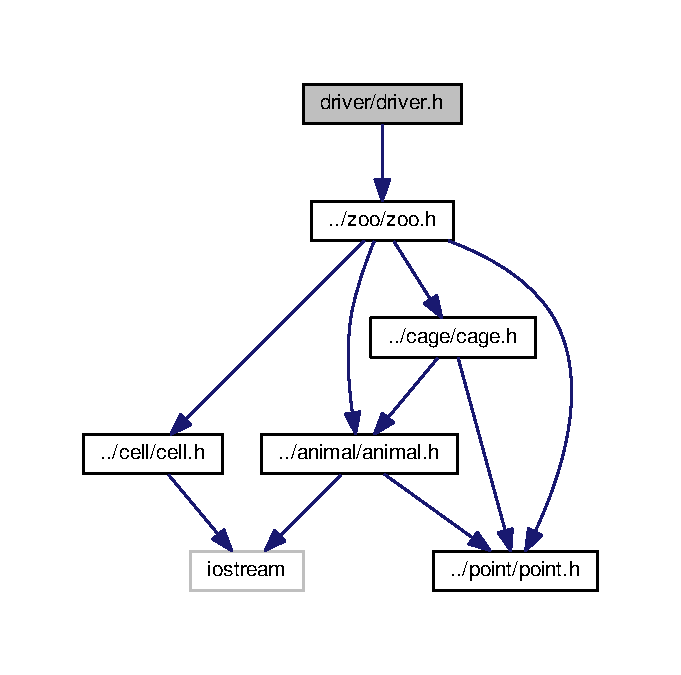
\includegraphics[width=327pt]{driver_8h__incl}
\end{center}
\end{figure}
This graph shows which files directly or indirectly include this file\+:\nopagebreak
\begin{figure}[H]
\begin{center}
\leavevmode
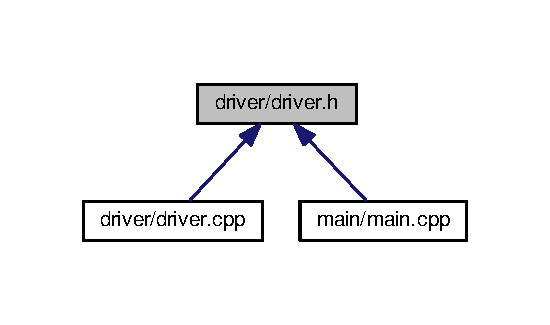
\includegraphics[width=264pt]{driver_8h__dep__incl}
\end{center}
\end{figure}
\subsection*{Classes}
\begin{DoxyCompactItemize}
\item 
class \hyperlink{classDriver}{Driver}
\end{DoxyCompactItemize}

\hypertarget{main_8cpp}{}\section{main.\+cpp File Reference}
\label{main_8cpp}\index{main.\+cpp@{main.\+cpp}}
{\ttfamily \#include \char`\"{}habitat.\+h\char`\"{}}\\*
{\ttfamily \#include \char`\"{}land\+\_\+habitat.\+h\char`\"{}}\\*
{\ttfamily \#include \char`\"{}water\+\_\+habitat.\+h\char`\"{}}\\*
{\ttfamily \#include \char`\"{}air\+\_\+habitat.\+h\char`\"{}}\\*
{\ttfamily \#include $<$iostream$>$}\\*
{\ttfamily \#include \char`\"{}driver.\+h\char`\"{}}\\*
Include dependency graph for main.\+cpp\+:
\nopagebreak
\begin{figure}[H]
\begin{center}
\leavevmode
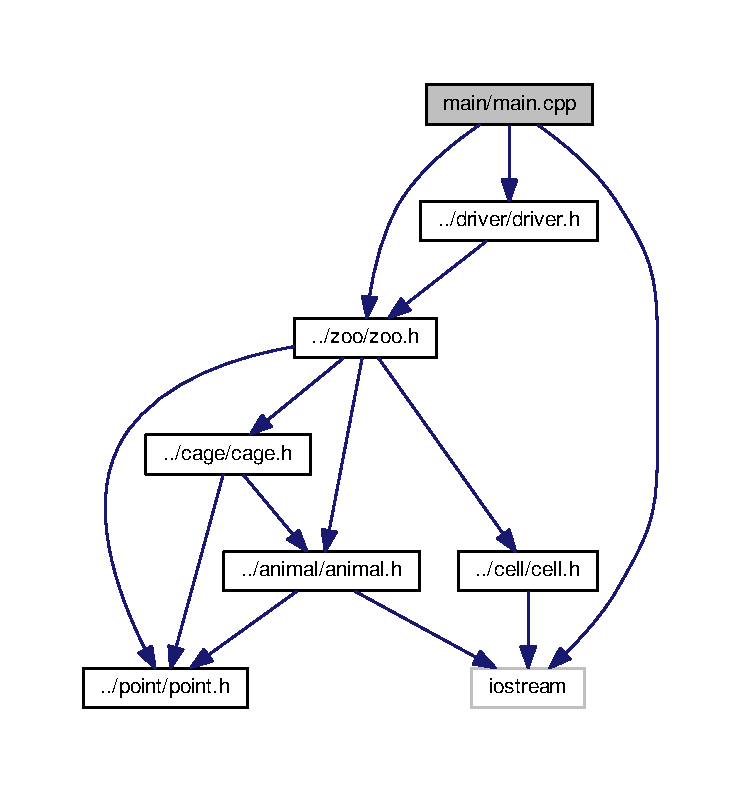
\includegraphics[width=350pt]{main_8cpp__incl}
\end{center}
\end{figure}
\subsection*{Functions}
\begin{DoxyCompactItemize}
\item 
int \hyperlink{main_8cpp_ae66f6b31b5ad750f1fe042a706a4e3d4}{main} ()
\end{DoxyCompactItemize}


\subsection{Function Documentation}
\index{main.\+cpp@{main.\+cpp}!main@{main}}
\index{main@{main}!main.\+cpp@{main.\+cpp}}
\subsubsection[{\texorpdfstring{main()}{main()}}]{\setlength{\rightskip}{0pt plus 5cm}int main (
\begin{DoxyParamCaption}
{}
\end{DoxyParamCaption}
)}\hypertarget{main_8cpp_ae66f6b31b5ad750f1fe042a706a4e3d4}{}\label{main_8cpp_ae66f6b31b5ad750f1fe042a706a4e3d4}

\hypertarget{map_8txt}{}\section{map.\+txt File Reference}
\label{map_8txt}\index{map.\+txt@{map.\+txt}}

\hypertarget{point_8cpp}{}\section{point/point.cpp File Reference}
\label{point_8cpp}\index{point/point.\+cpp@{point/point.\+cpp}}
{\ttfamily \#include \char`\"{}../point/point.\+h\char`\"{}}\\*
Include dependency graph for point.\+cpp\+:
\nopagebreak
\begin{figure}[H]
\begin{center}
\leavevmode
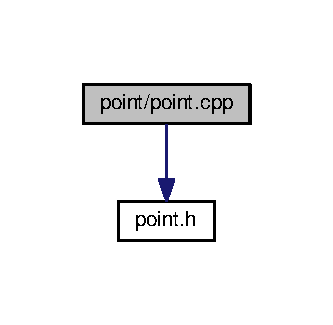
\includegraphics[width=160pt]{point_8cpp__incl}
\end{center}
\end{figure}

\hypertarget{point_8h}{}\section{point/point.h File Reference}
\label{point_8h}\index{point/point.\+h@{point/point.\+h}}
This graph shows which files directly or indirectly include this file\+:
% FIG 0
\subsection*{Classes}
\begin{DoxyCompactItemize}
\item 
class \hyperlink{classPoint}{Point}
\end{DoxyCompactItemize}

\hypertarget{zoo_8cpp}{}\section{zoo.\+cpp File Reference}
\label{zoo_8cpp}\index{zoo.\+cpp@{zoo.\+cpp}}
{\ttfamily \#include \char`\"{}zoo.\+h\char`\"{}}\\*
{\ttfamily \#include $<$iostream$>$}\\*
{\ttfamily \#include $<$fstream$>$}\\*
Include dependency graph for zoo.\+cpp\+:
\nopagebreak
\begin{figure}[H]
\begin{center}
\leavevmode
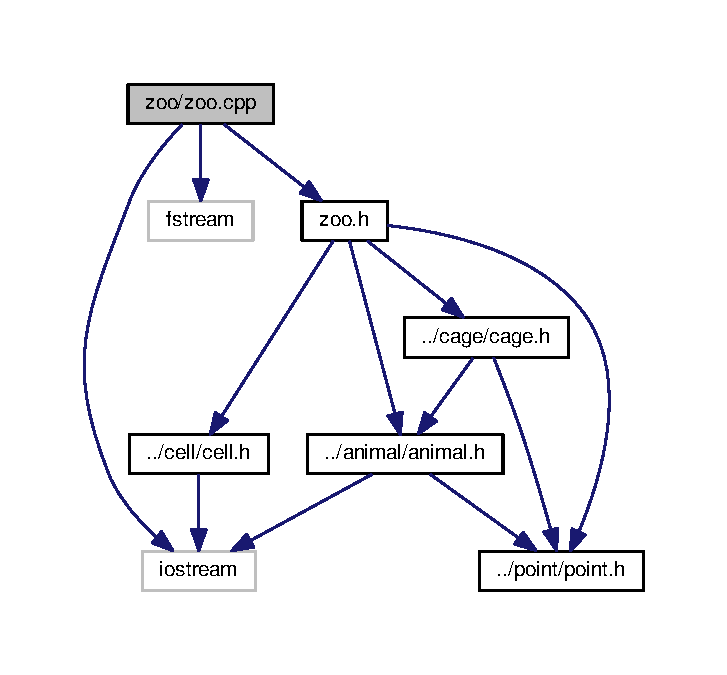
\includegraphics[width=350pt]{zoo_8cpp__incl}
\end{center}
\end{figure}
\subsection*{Functions}
\begin{DoxyCompactItemize}
\item 
ostream \& \hyperlink{zoo_8cpp_a9a5a25ae9291345b74f5d8f7af9719db}{operator$<$$<$} (ostream \&o, const \hyperlink{classZoo}{Zoo} \&z)
\item 
istream \& \hyperlink{zoo_8cpp_a66565ea7c66ddb3acdcb0b67930b8615}{operator$>$$>$} (istream \&is, \hyperlink{classZoo}{Zoo} \&z)
\end{DoxyCompactItemize}


\subsection{Function Documentation}
\index{zoo.\+cpp@{zoo.\+cpp}!operator$<$$<$@{operator$<$$<$}}
\index{operator$<$$<$@{operator$<$$<$}!zoo.\+cpp@{zoo.\+cpp}}
\subsubsection[{\texorpdfstring{operator$<$$<$(ostream \&o, const Zoo \&z)}{operator<<(ostream &o, const Zoo &z)}}]{\setlength{\rightskip}{0pt plus 5cm}ostream\& operator$<$$<$ (
\begin{DoxyParamCaption}
\item[{ostream \&}]{o, }
\item[{const {\bf Zoo} \&}]{z}
\end{DoxyParamCaption}
)}\hypertarget{zoo_8cpp_a9a5a25ae9291345b74f5d8f7af9719db}{}\label{zoo_8cpp_a9a5a25ae9291345b74f5d8f7af9719db}

\begin{DoxyParams}{Parameters}
{\em o} & Objek ostream. \\
\hline
{\em z} & Objek \hyperlink{classZoo}{Zoo} yang akan dicetak. \\
\hline
\end{DoxyParams}
\begin{DoxyReturn}{Returns}
Menghasilkan objek ostream yang akan dicetak. 
\end{DoxyReturn}
\index{zoo.\+cpp@{zoo.\+cpp}!operator$>$$>$@{operator$>$$>$}}
\index{operator$>$$>$@{operator$>$$>$}!zoo.\+cpp@{zoo.\+cpp}}
\subsubsection[{\texorpdfstring{operator$>$$>$(istream \&is, Zoo \&z)}{operator>>(istream &is, Zoo &z)}}]{\setlength{\rightskip}{0pt plus 5cm}istream\& operator$>$$>$ (
\begin{DoxyParamCaption}
\item[{istream \&}]{is, }
\item[{{\bf Zoo} \&}]{z}
\end{DoxyParamCaption}
)}\hypertarget{zoo_8cpp_a66565ea7c66ddb3acdcb0b67930b8615}{}\label{zoo_8cpp_a66565ea7c66ddb3acdcb0b67930b8615}

\begin{DoxyParams}{Parameters}
{\em i} & Objek istream. \\
\hline
{\em z} & Objek \hyperlink{classZoo}{Zoo} yang akan dibaca. \\
\hline
\end{DoxyParams}
\begin{DoxyReturn}{Returns}
Mengeluarkan objek istream yang telah dibaca. 
\end{DoxyReturn}

\hypertarget{zoo_8h}{}\section{zoo/zoo.h File Reference}
\label{zoo_8h}\index{zoo/zoo.\+h@{zoo/zoo.\+h}}
{\ttfamily \#include \char`\"{}../cell/cell.\+h\char`\"{}}\\*
{\ttfamily \#include \char`\"{}../cage/cage.\+h\char`\"{}}\\*
{\ttfamily \#include \char`\"{}../point/point.\+h\char`\"{}}\\*
{\ttfamily \#include \char`\"{}../animal/animal.\+h\char`\"{}}\\*
{\ttfamily \#include \char`\"{}../land\+\_\+habitat/land\+\_\+habitat.\+h\char`\"{}}\\*
{\ttfamily \#include \char`\"{}../water\+\_\+habitat/water\+\_\+habitat.\+h\char`\"{}}\\*
{\ttfamily \#include \char`\"{}../air\+\_\+habitat/air\+\_\+habitat.\+h\char`\"{}}\\*
{\ttfamily \#include \char`\"{}../restaurant/restaurant.\+h\char`\"{}}\\*
{\ttfamily \#include \char`\"{}../park/park.\+h\char`\"{}}\\*
{\ttfamily \#include \char`\"{}../road/road.\+h\char`\"{}}\\*
{\ttfamily \#include \char`\"{}../exit/exit.\+h\char`\"{}}\\*
{\ttfamily \#include \char`\"{}../entrance/entrance.\+h\char`\"{}}\\*
{\ttfamily \#include \char`\"{}../alligator/alligator.\+h\char`\"{}}\\*
{\ttfamily \#include \char`\"{}../cobra/cobra.\+h\char`\"{}}\\*
{\ttfamily \#include \char`\"{}../cormorant/cormorant.\+h\char`\"{}}\\*
{\ttfamily \#include \char`\"{}../dolphin/dolphin.\+h\char`\"{}}\\*
{\ttfamily \#include \char`\"{}../duck/duck.\+h\char`\"{}}\\*
{\ttfamily \#include \char`\"{}../dugong/dugong.\+h\char`\"{}}\\*
{\ttfamily \#include \char`\"{}../eagle/eagle.\+h\char`\"{}}\\*
{\ttfamily \#include \char`\"{}../elephant/elephant.\+h\char`\"{}}\\*
{\ttfamily \#include \char`\"{}../giraffe/giraffe.\+h\char`\"{}}\\*
{\ttfamily \#include \char`\"{}../goat/goat.\+h\char`\"{}}\\*
{\ttfamily \#include \char`\"{}../iguana/iguana.\+h\char`\"{}}\\*
{\ttfamily \#include \char`\"{}../jalak/jalak.\+h\char`\"{}}\\*
{\ttfamily \#include \char`\"{}../komodo/komodo.\+h\char`\"{}}\\*
{\ttfamily \#include \char`\"{}../lion/lion.\+h\char`\"{}}\\*
{\ttfamily \#include \char`\"{}../orca/orca.\+h\char`\"{}}\\*
{\ttfamily \#include \char`\"{}../owl/owl.\+h\char`\"{}}\\*
{\ttfamily \#include \char`\"{}../parrot/parrot.\+h\char`\"{}}\\*
{\ttfamily \#include \char`\"{}../polar\+\_\+bear/polar\+\_\+bear.\+h\char`\"{}}\\*
{\ttfamily \#include \char`\"{}../tiger/tiger.\+h\char`\"{}}\\*
{\ttfamily \#include \char`\"{}../walrus/walrus.\+h\char`\"{}}\\*
Include dependency graph for zoo.\+h\+:
% FIG 0
This graph shows which files directly or indirectly include this file\+:
% FIG 1
\subsection*{Classes}
\begin{DoxyCompactItemize}
\item 
class \hyperlink{classZoo}{Zoo}
\end{DoxyCompactItemize}

%--- End generated contents ---

% Index
\backmatter
\newpage
\phantomsection
\clearemptydoublepage
\addcontentsline{toc}{chapter}{Index}
\printindex

\end{document}
